\documentclass[aspectratio=169]{beamer}
\usepackage[utf8]{inputenc}
\usepackage[T5]{fontenc}
\usepackage{vietnam}
\usepackage{amsmath}
\usepackage{amssymb}
\usepackage{graphicx}
\usepackage{booktabs}
\usepackage{algorithm}
\usepackage{algpseudocode}
\usepackage{multicol}
\usepackage{capt-of} % provides \captionof for captions outside float environments
\usepackage{animate}
\usepackage{multimedia}  % Thêm package để nhúng video
\usepackage{tikz} % Để vẽ minh họa hoặc chèn hình

\usepackage[vietnamese]{babel}
\usepackage{caption}
\usepackage{subcaption}
\usetheme{Madrid}
\usecolortheme{default}

% Tùy chỉnh màu sắc title page
\setbeamercolor{title}{fg=blue!80!cyan}
\setbeamercolor{subtitle}{fg=blue!60!black}
\setbeamercolor{author}{fg=black!80}
\setbeamercolor{institute}{fg=black!60}
\setbeamercolor{date}{fg=black!60}

% Logo ở góc trên bên phải mọi slide
% \usepackage{tikz}

% \addtobeamertemplate{headline}{}{
%     \begin{tikzpicture}[remember picture,overlay]
%         \node [anchor=north east, xshift=-0.2cm, yshift=-1cm] at (current page.north east) {
%             
\includegraphics[height=1cm]{./imgs/logo.png}
%         };
%     \end{tikzpicture}
% }

% Tùy chỉnh footer ngắn gọn
\setbeamertemplate{footline}
{
  \leavevmode%
  \hbox{%
  \begin{beamercolorbox}[wd=.33\paperwidth,ht=2.25ex,dp=1ex,center]{author in head/foot}%
    \usebeamerfont{author in head/foot}\insertshortauthor
  \end{beamercolorbox}%
  \begin{beamercolorbox}[wd=.34\paperwidth,ht=2.25ex,dp=1ex,center]{title in head/foot}%
    \usebeamerfont{title in head/foot}\insertshorttitle
  \end{beamercolorbox}%
  \begin{beamercolorbox}[wd=.33\paperwidth,ht=2.25ex,dp=1ex,right]{date in head/foot}%
    \usebeamerfont{date in head/foot}\insertshortdate{}\hspace*{2em}
    \insertframenumber{} / \inserttotalframenumber\hspace*{2ex} 
  \end{beamercolorbox}}%
  \vskip0pt%
}

% Tùy chỉnh màu sắc cho các box
\setbeamercolor{block title}{bg=blue!70,fg=white}
\setbeamercolor{block body}{bg=blue!10,fg=black}
\setbeamercolor{block title alerted}{bg=red!70,fg=white}
\setbeamercolor{block body alerted}{bg=red!10,fg=black}
\setbeamercolor{block title example}{bg=teal!60,fg=white}
\setbeamercolor{block body example}{bg=teal!8,fg=black}

% \institute{
%     Trường Đại học Bách Khoa - ĐHQG TP.HCM \\
%     Khoa Khoa học và Kỹ thuật Máy tính
% }
% \title{\textcolor{black!}{\textbf{Hoạch định chuyển động quanh chướng ngại vật bằng tối ưu lồi}}}
% \author{
%     \textbf{Nguyen Tran Dang Khoa} - 2211635 \\
%     \textbf{Ho Dang Khoa} - 2211588 \\[1em]
%     {\small GVHD: PGS.TS. Le Hong Trang}
% }
% % Định nghĩa phiên bản ngắn cho footer
% \author[Khoa N.T.D. \& Khoa H.D.]{
%     \textbf{Nguyen Tran Dang Khoa} - 2211635 \\
%     \textbf{Ho Dang Khoa} - 2211588 \\[1em]
%     {\small GVHD: PGS.TS. Le Hong Trang}
% }
% \title[Motion Planning - GCS]{\textcolor{black!}{\textbf{Hoạch định chuyển động quanh chướng ngại vật bằng tối ưu lồi}}}
% \date[\today]{\today}

\begin{document}

% Trang title tùy chỉnh
% {
% \setbeamertemplate{headline}{} % Tắt header
% \setbeamertemplate{footline}{} % Tắt footer
% \begin{frame}
%     \titlepage
% \end{frame}
% }

% --- TRANG GIỚI THIỆU TÙY CHỈNH (REDESIGN) ---
\begin{frame}[plain]
    \centering

    % Header: Trường / Khoa
    {\footnotesize\bfseries
        ĐẠI HỌC QUỐC GIA TP.HCM\\
        TRƯỜNG ĐẠI HỌC BÁCH KHOA\\
        KHOA KHOA HỌC VÀ KỸ THUẬT MÁY TÍNH
    }

    \vspace{0.35cm}

    % Logos (thêm 1 logo bên trái)
    \begin{minipage}{\textwidth}
        \centering
        
\includegraphics[width=3.0cm]{./imgs/Logo DHQG-HCM khong nen_2.png}\hspace{0.6cm}%
        
\includegraphics[width=1.5cm]{./imgs/LogoBK.png}
    \end{minipage}

    % \vspace{0.35cm}

    % Title block
    \begin{beamercolorbox}[wd=\textwidth,sep=5pt,center,rounded=true,shadow=true]{block title}
        {\Large\bfseries Hoạch định chuyển động của rô-bốt}\\[-1mm]
        {\Large\bfseries sử dụng tối ưu lồi}
    \end{beamercolorbox}

    \vspace{0.25cm}

    {\small\bfseries HK252-DATN-028}

    % \vspace{0.35cm}

    \rule{0.85\textwidth}{0.4pt}

    % \vspace{0.35cm}

    % Supervisors / Students
    \begin{columns}[T,onlytextwidth]
        \begin{column}{0.52\textwidth}
            \centering
            {\footnotesize\bfseries Người hướng dẫn:}\\[2pt]
            {\footnotesize
            PGS. TS. Lê Hồng Trang\\
            Ths. Trương Quỳnh Chi
            }
        \end{column}
        \begin{column}{0.48\textwidth}
            \centering
            {\footnotesize\bfseries Sinh viên:}\\[2pt]
            {\footnotesize
            Hồ Đăng Khoa (2211588)\\
            Nguyễn Trần Đăng Khoa (2211635)
            }
        \end{column}
    \end{columns}

    \vspace*{\fill}

    % Footer: Địa điểm / thời gian
    {\footnotesize Hồ Chí Minh, \today}
\end{frame}

\begin{frame}{Tổng quan}
    \tableofcontents
\end{frame}

\section{Giới thiệu}

\begin{frame}{Động lực}

    \begin{center}
        \fbox{\parbox{0.9\textwidth}{%
                Trọng tâm của các bài toán rô-bốt là tối ưu các quyết định rời rạc cấp cao và quyết định liên tục cấp thấp.
            }}
    \end{center}

    % Ảnh
    \begin{columns}[T,onlytextwidth]
        \begin{column}{0.5\textwidth}
            \centering
            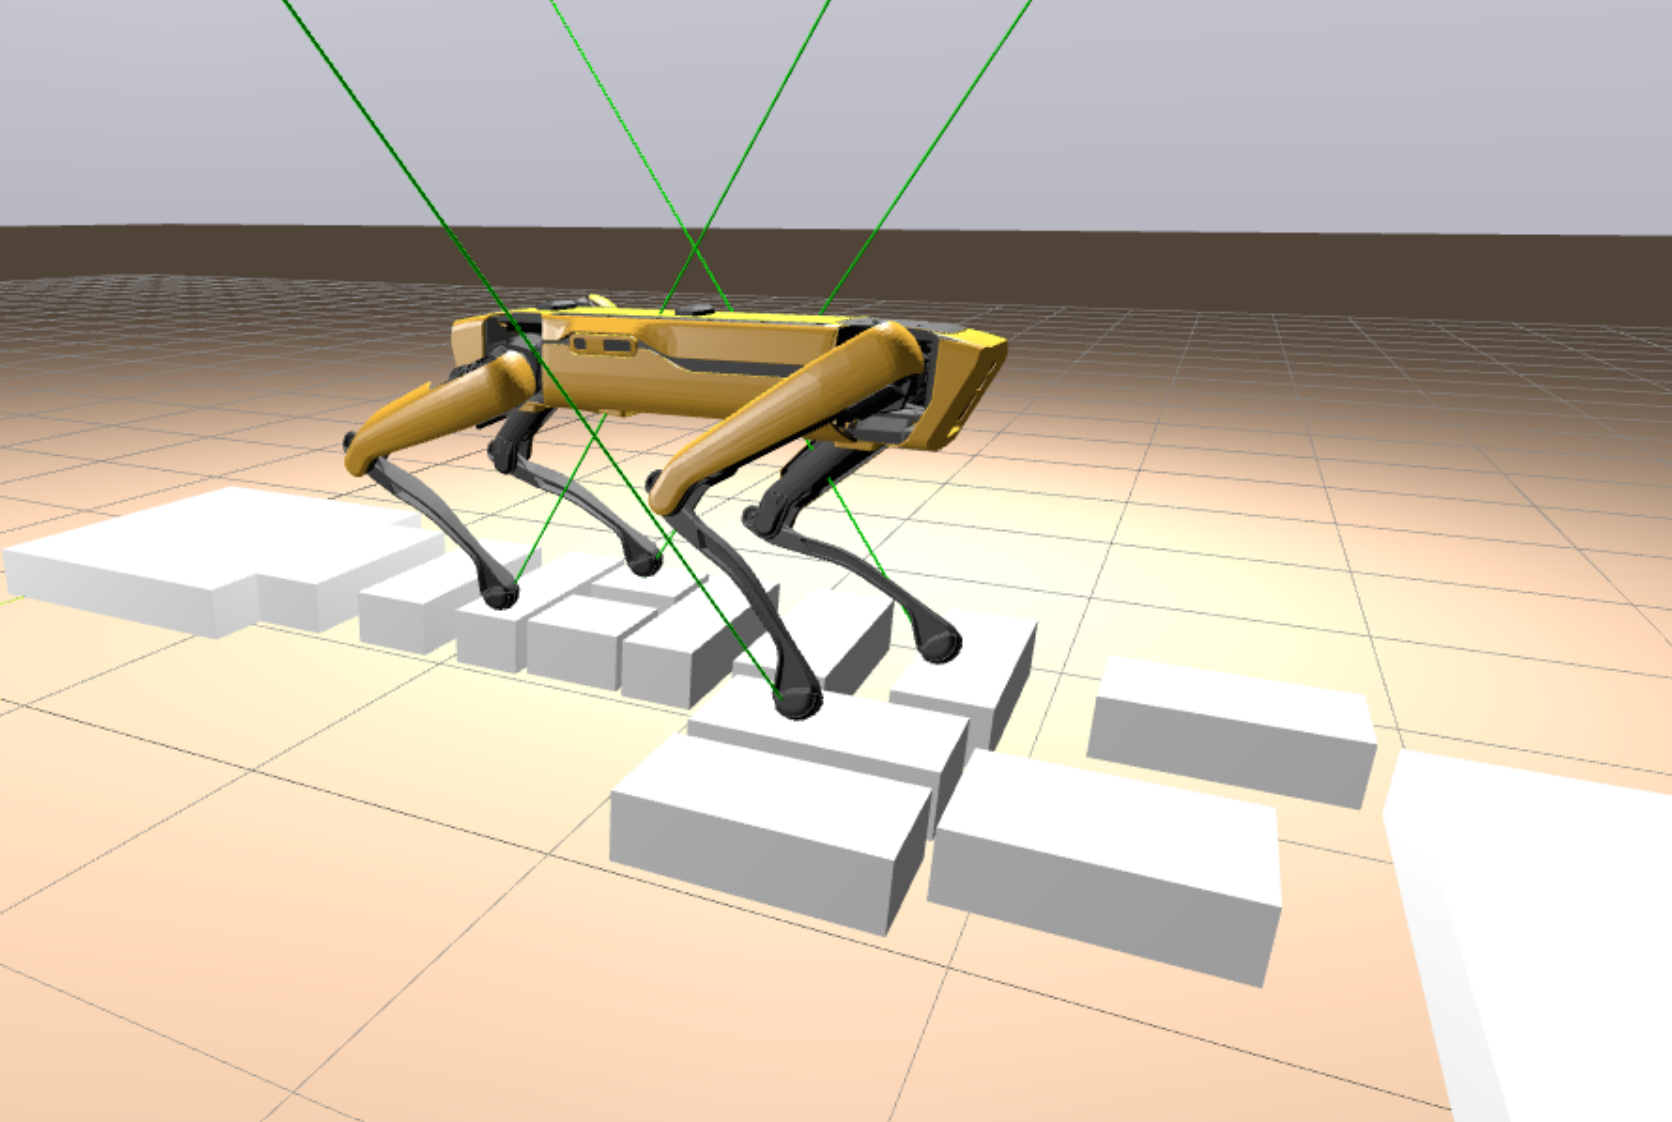
\includegraphics[width=0.7\linewidth]{./imgs/dog-robot.png}
            \captionof{figure}{Rô-bốt chó đi qua địa hình phức tạp\footnotemark}
        \end{column}
        \begin{column}{0.5\textwidth}
            \centering
            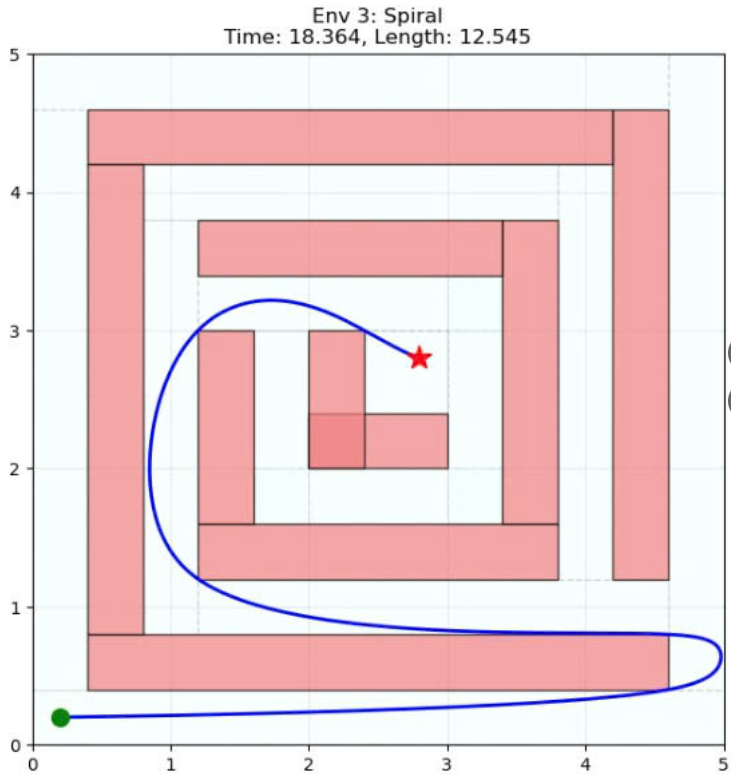
\includegraphics[width=0.4\linewidth]{./imgs/bezier-env3-2.png}
            \captionof{figure}{Quỹ đạo tối ưu trong mê cung}
        \end{column}
    \end{columns}

    \footnotetext{Nguồn: Johannes Ihle et al., ``Graph of Convex Sets for Trajectory Optimization on Spot''}
\end{frame}

\begin{frame}{Bài toán hoạch định chuyển động}
    \begin{columns}[T]
        \begin{column}{0.35\textwidth}
            % \begin{definition}[Bài toán Motion Planning]
            %     Tìm quỹ đạo khả thi cho robot di chuyển từ cấu hình đầu $q_{\text{start}}$ đến cấu hình đích $q_{\text{goal}}$ trong môi trường có chướng ngại vật, thỏa mãn các ràng buộc vật lý và động lực học.
            % \end{definition}

            % \vspace{0.3cm}
            % \textbf{Thách thức chính:}
            % \begin{itemize}
            %     \item Tránh va chạm 
            %     \item Ràng buộc động lực học
            %     \item Tối ưu hóa 
            %     \item Độ phức tạp tính toán 
            % \end{itemize}
            \begin{block}{Định nghĩa bài toán}
                \begin{itemize}
                    \item \textbf{Đầu vào:} $x_{\text{start}}$ (vị trí/vận tốc/\ldots), $x_{\text{goal}}$, vật cản
                    \item \textbf{Đầu ra:} quỹ đạo $x(t)$ / chuỗi điều khiển $u(t)$
                    \item \textbf{Mục tiêu:} không va chạm, trơn, tối ưu chi phí.
                    \item \textbf{Ràng buộc:} động, giới hạn (state/control).
                \end{itemize}
            \end{block}
        \end{column}

        \begin{column}{0.65\textwidth}
            \centering
            % Video nhúng - cần file video.mp4 trong thư mục
            \begin{figure}
                % \rotatebox{90}{
                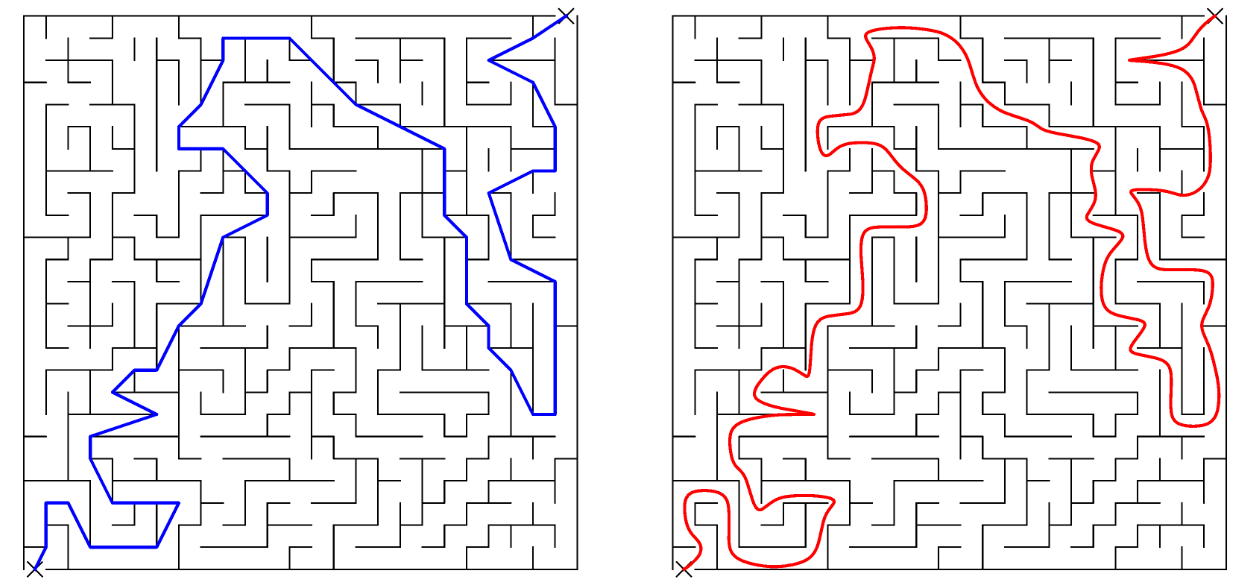
\includegraphics[width=0.9\textwidth]{./imgs/motion-path.png}
                % }
                \caption{Path planning (bên trái) và Motion planning (bên phải)}
            \end{figure}
        \end{column}
    \end{columns}
\end{frame}

% \begin{frame}{Phương pháp hoạch định chuyển động}
%     \begin{columns}[T]
%         \begin{column}{0.5\textwidth}
%             \textbf{Sampling-based methods:}
%             \begin{itemize}
%                 \item RRT (Rapidly-exploring Random Tree)
%                 \item RRT* (optimal variant)
%                 \item PRM (Probabilistic Roadmap)
%             \end{itemize}
%             \textit{Ưu:} Nhanh, mở rộng tốt\\
%             \textit{Nhược:} Không đảm bảo tối ưu, quỹ đạo không trơn

%         \end{column}

%         \begin{column}{0.5\textwidth}
%             \animategraphics[autoplay,loop,width=0.9\textwidth]{20}{./imgs/RRT-}{0}{296}
%         \end{column}
%     \end{columns}

% \end{frame}

\begin{frame}{Bài toán hoạch định chuyển động}
    \begin{columns}[T,onlytextwidth]
        \begin{column}{0.33\textwidth}
            \centering
            \small
            \textbf{Truyền thống:}
            \begin{itemize}
                \item Đường đi ngắn nhất (A-star, Dijkstra)
                \item Tối ưu hóa quỹ đạo
            \end{itemize}
            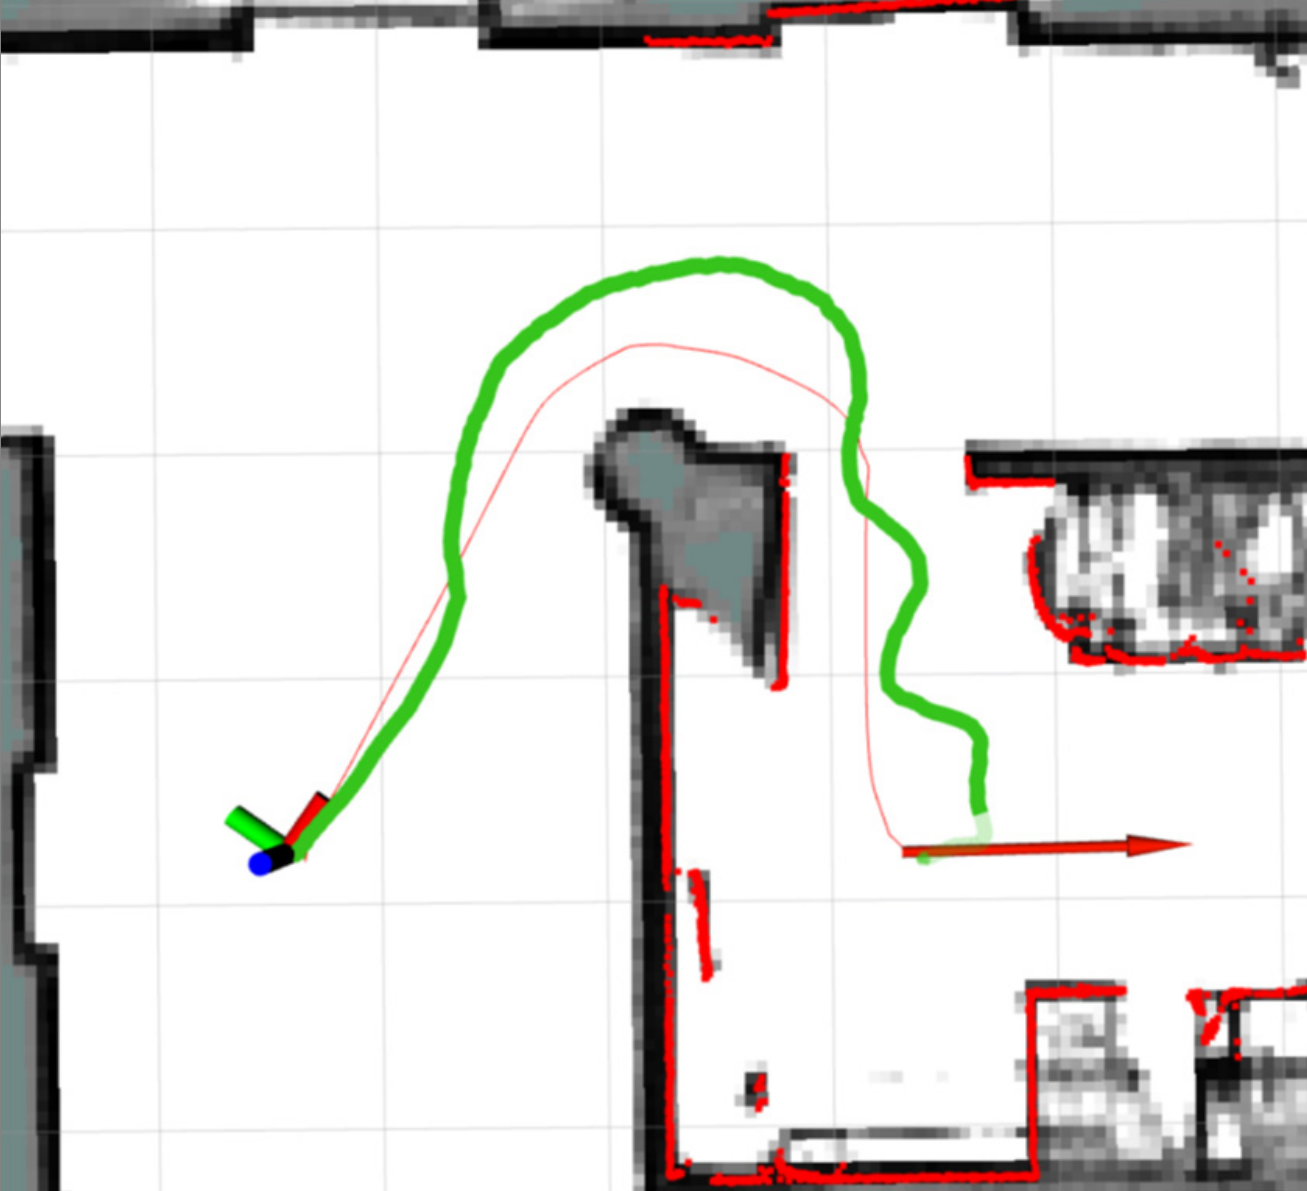
\includegraphics[width=0.7\linewidth]{./imgs/Screenshot 2025-12-26 230008.png}
            \captionof{figure}{Decoupling methods\footnotemark}
        \end{column}
        \begin{column}{0.33\textwidth}
            \centering
            \textbf{Phương pháp Sampling-based:}
            \begin{itemize}
                \small
                \item RRT (Rapidly-exploring Random Tree)
                % \item RRT* (optimal variant)
                \item PRM (Probabilistic Roadmap)
            \end{itemize}
            \begin{figure}
                {
                    \centering
                    % \textbf{RRT}~\cite{lavalle1998}
                    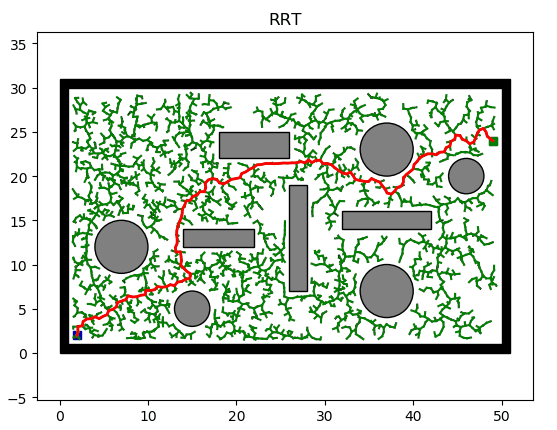
\includegraphics[width=0.8\linewidth]{./imgs/RRT/RRT-296}
                }
            \end{figure}
        \end{column}
        \begin{column}{0.33\textwidth}
            \centering
            \textbf{SPP in GCS Framework}~\cite{marcucci2023motion, marcucci2024shortest}
            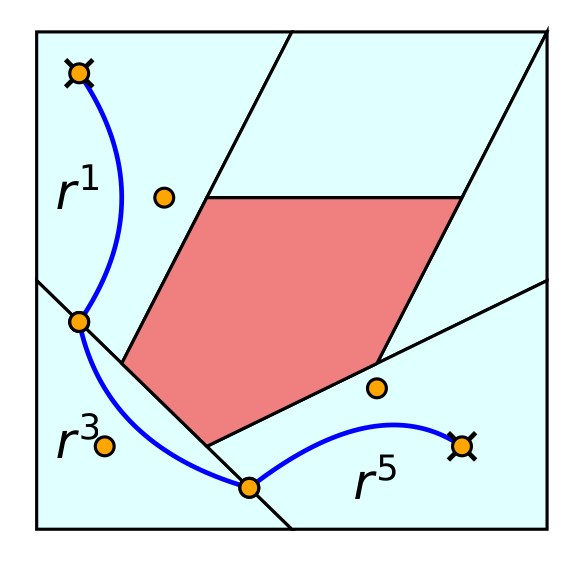
\includegraphics[width=\linewidth]{./imgs/gcs-example.png}
        \end{column}
    \end{columns}
    \footnotetext{Nguồn: Aditya Tandon et al, ``Autonomous navigation of quadruped robots for monitoring and inspection of civil infrastructure ''}
\end{frame}

\section{Graph of Convex Sets (GCS)}

\begin{frame}{Ý tưởng chính (GCS)}
    \begin{itemize}
        \item \textbf{Phân hoạch không gian:} $\rightarrow$ \textbf{vùng an toàn lồi} $\{Q_v\}$
        \item \textbf{Mô hình hóa:} Hoạch định chuyển động $\rightarrow$ \textbf{SPP} trên \textbf{Graph of Convex Sets}
        \item \textbf{Quyết định:}
              \begin{itemize}
                  \item \textbf{Rời rạc:} chọn cạnh / đường đi
                  \item \textbf{Liên tục:} trạng thái / quỹ đạo trong $Q_v$
              \end{itemize}
        \item \textbf{Giải:} \textbf{relaxation} $\rightarrow$ convex optimization $\rightarrow$ đường khả thi tối ưu toàn cục
    \end{itemize}

    \begin{block}{Convex safe region}
        $Q_v \subset \mathbb{R}^n$: lồi, đóng, an toàn~\cite{marcucci2023motion}.
    \end{block}
    \centering
    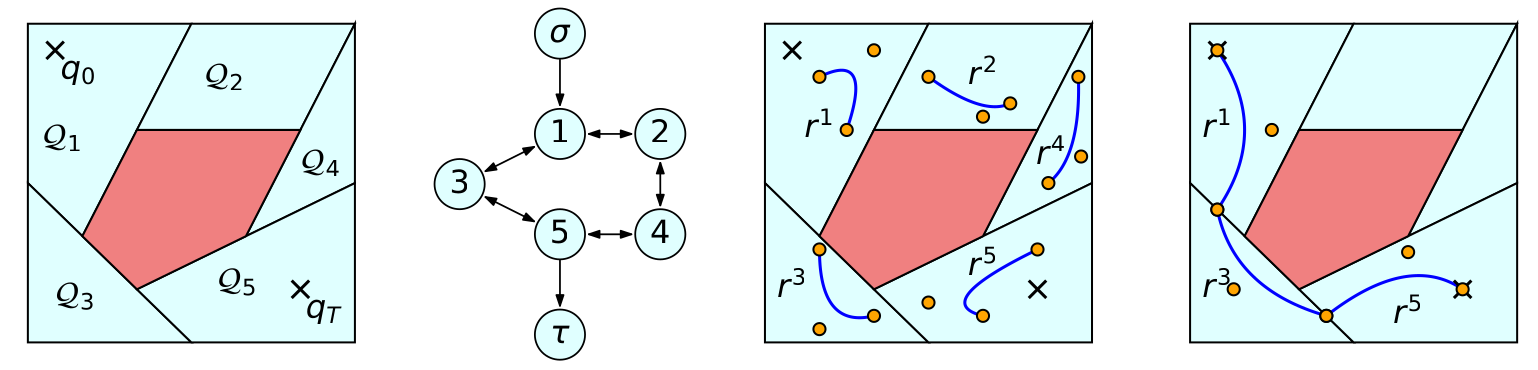
\includegraphics[width=0.8\linewidth]{./imgs/pipeline-GCS.png}
\end{frame}

% \begin{frame}{Cấu trúc đồ thị GCS}
%     Đồ thị của các tập lồi là sự tổng quát hóa của một đồ thị có hướng. Cụ thể gọi $G = (V, \mathcal{E})$ là đồ thị có hướng, trong đó: \\
%     \vspace{0.5em}
%     \textbf{Thành phần Đỉnh (Vertices):} Mỗi đỉnh $v \in V$ ứng với
%     \begin{itemize}
%         \item Một vùng an toàn lồi $Q_v$
%         \item Biến liên tục $x_v \in \mathbb{R}^{n_v}$. Các biến liên tục $x_v$ phải nằm
%               trong tập lồi $\mathcal{X}_v \subset \mathbb{R}^{n_v}$ bao đóng (compact)
%     \end{itemize}
%     Về mặt toán học $x_v$ biểu diễn một điểm hoặc một vector cấu hình trạng thái được đại diện bởi đỉnh $v$. Số chiều $n_v$ ngụ ý mỗi đỉnh có thể có số chiều khác nhau.
% \end{frame}

% \begin{frame}{Cấu trúc đồ thị GCS}

%     \textbf{Cạnh (Edges):} Mỗi cạnh $e = [u, v] \in \mathcal{E}$ nối hai đỉnh $u, v \in V$ có các đặc điểm sau:
%     \begin{itemize}
%         \item Tồn tại một cạnh nối hai đỉnh $u$ và $v$ nếu thỏa mãn chính sách (ví dụ $Q_u
%                   \cap Q_v \neq \emptyset$)
%         \item Hàm chi phí cạnh
%               $\ell_e(x_u,x_v):\mathcal{X}_u\times\mathcal{X}_v\to[0,\infty]$ là một hàm lồi,
%               đóng và thực (proper). Chi phí này phụ thuộc vào các biến liên tục
%               $x_u\in\mathcal{X}_u$ và $x_v\in\mathcal{X}_v$ tại hai đỉnh $u$ và $v$.
%         \item Với mỗi cạnh $e = [v, w] \in \mathcal{E}$, tồn tại một Tập ràng buộc liên kết
%               $\mathcal{X}_e \subseteq \mathbb{R}^{n_v + n_w}$ chứa tất cả các cặp biến
%               $(x_v, x_w)$ thỏa mãn ràng buộc liên kết giữa hai đỉnh $v$ và $w$.
%     \end{itemize}
%     Lưu ý: $\ell_e$ đại diện cho chi phí tổng quát, không bắt buộc là một metric (tức là không cần tính đối xứng hay bất đẳng thức tam giác).~\cite{marcucci2023motion}

% \end{frame}

\begin{frame}{Phân hoạch không gian an toàn lồi}
    \begin{columns}[T,onlytextwidth]
        \begin{column}{0.5\textwidth}
            \centering

            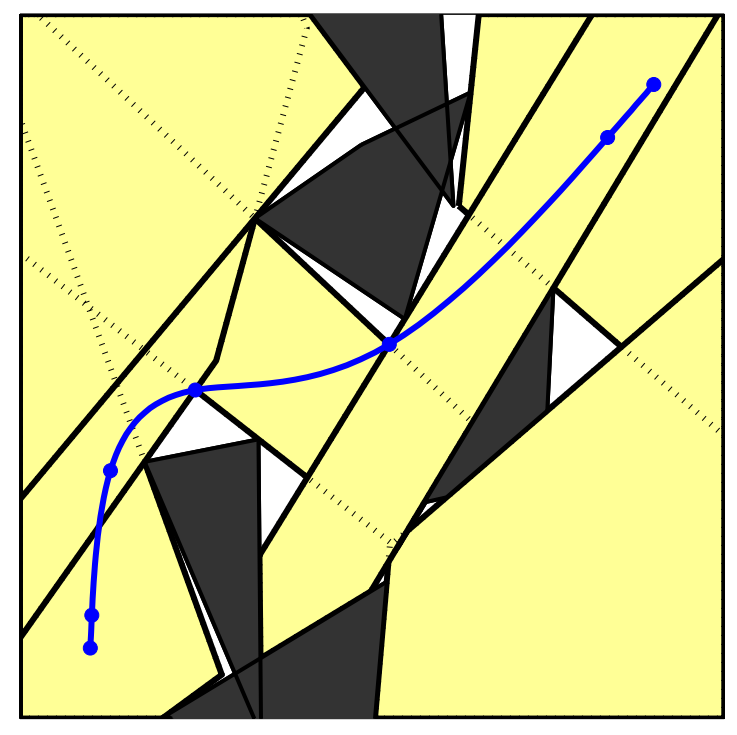
\includegraphics[width=0.8\linewidth]{./imgs/decompose-ex-2.png}
            \captionof{figure}{Phân hoạch không gian an toàn lồi~\cite{marcucci2023motion}}
        \end{column}
        \begin{column}{0.5\textwidth}
            \begin{block}{Phân hoạch lồi (Convex Decomposition)}
                \textbf{Phân hoạch lồi} là quá trình chia một hình học phức tạp (không lồi) thành một tập hợp các \textbf{vùng con lồi}.
            \end{block}

            \vspace{0.5em}

            \textbf{Mục tiêu:}
            \begin{itemize}
                \item Tối thiểu hóa số lượng vùng lồi, vùng lồi lớn nhất có thể.
                \item Các vùng lồi con bao toàn bộ không gian.
            \end{itemize}

            \textbf{Ý nghĩa:}
            \begin{itemize}
                \item Tạo ra các vùng tránh vật cản.
                \item Tiền đề cho mô hình hóa.
            \end{itemize}
        \end{column}
    \end{columns}
\end{frame}

\begin{frame}{Một số giải thuật phân hoạch lồi}
    \begin{columns}[T,onlytextwidth]
        \begin{column}{0.50\textwidth}
            \textbf{Giải thuật phổ biến:}
            \begin{itemize}
                \item \textbf{Phân hoạch chính xác:}
                      \begin{itemize}
                          \item Giải thuật quét hình thang (Sweeping Trapezoidation)~\cite{ecd_lectures}
                          \item Giải thuật ngẫu nhiên của Seidel~\cite{seidel_decompose}
                      \end{itemize}
                \item \textbf{Phân hoạch xấp xỉ:}
                      \begin{itemize}
                          \item VCC (Visibility Clique Cover)~\cite{vcc2023}
                          \item ACD (Approximate Convex Decomposition)~\cite{lien1994approximate}
                      \end{itemize}
            \end{itemize}

        \end{column}

        \begin{column}{0.45\textwidth}
            \centering
            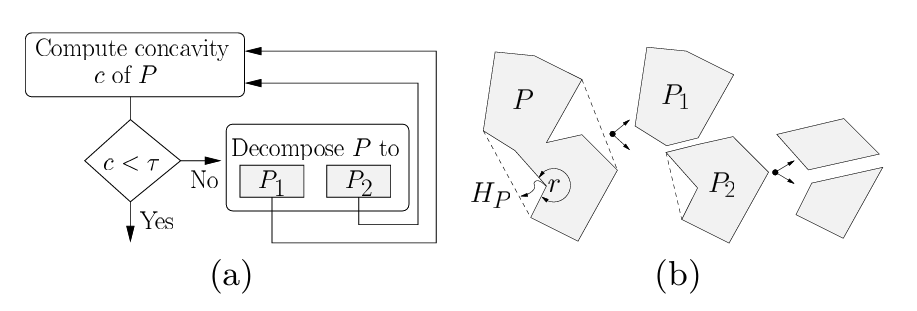
\includegraphics[width=\linewidth]{./imgs/ACD-1.png}
            \captionof{figure}{Giải thuật phân hoạch xấp xỉ ACD}
        \end{column}
    \end{columns}
    \vspace{0.5em}
    \centering
    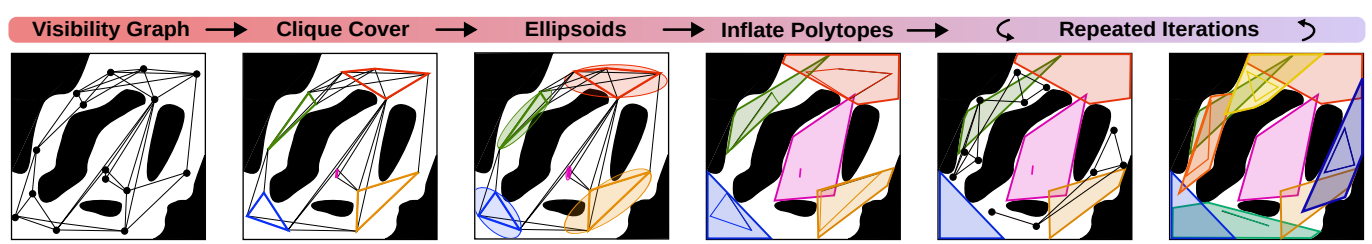
\includegraphics[width=\linewidth]{./imgs/VCC.png}
\end{frame}

\begin{frame}{Cấu trúc GCS (Graph of Convex Sets)}

    \begin{columns}[T,onlytextwidth]
        \begin{column}{0.5\textwidth}
            \textbf{GCS:} đồ thị có hướng $G=(V,\mathcal{E})$ \\
            \textbf{Đỉnh $v\in V$:}
            \begin{itemize}
                % \item \textbf{Vùng lồi} $Q_v$ (không va chạm, lồi)
                \item \textbf{Biến liên tục:} $x_v$ $\in X_v$
                \item \textbf{Tập lồi:} $X_v \subset R^{n_v}$ với $n_v$ chiều
            \end{itemize}
            \textbf{Cạnh $e=(u,v)\in\mathcal{E}$:}
            \begin{itemize}
                % \item \textbf{Chuyển tiếp} giữa $Q_u \leftrightarrow Q_v$
                \item \textbf{Hàm chi phí:} $\ell_e(x_u,x_v)$
                \item \textbf{Ràng buộc kết nối:} $(x_u,x_v)\in\mathcal{X}_e$
            \end{itemize}
        \end{column}
        \begin{column}{0.5\textwidth}
            \centering
            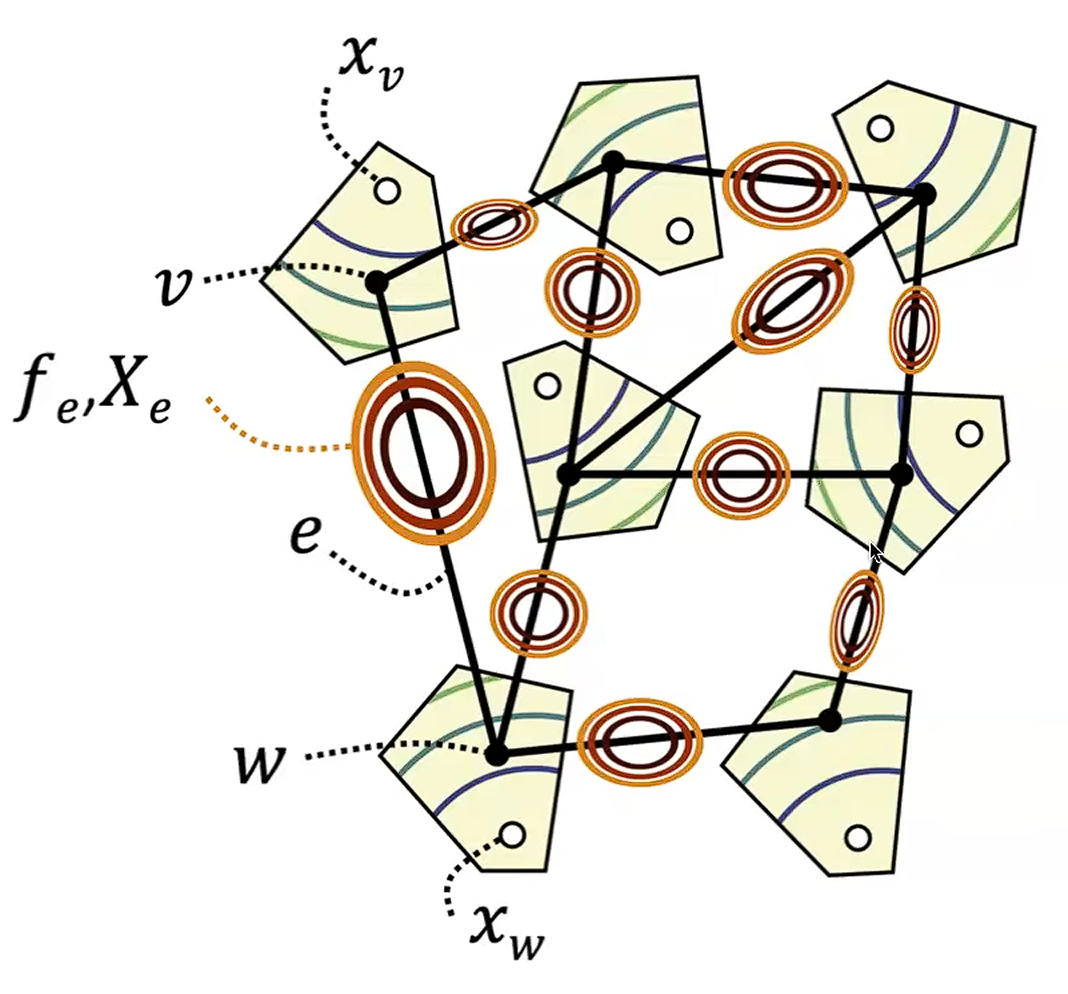
\includegraphics[width=0.8\linewidth]{./imgs/gcs-frame-1.png}
            \captionof{figure}{GCS Framework\footnotemark}
        \end{column}
    \end{columns}
    % Lưu ý: $\ell_e$ đại diện cho chi phí tổng quát, lồi đóng, không bắt buộc là một metric

    \footnotetext{Nguồn: Marcucci et al., ``Motion Planning around Obstacles with Convex Optimization''}
\end{frame}

\section{Bài toán tối ưu hóa}

\begin{frame}{Bài toán tìm đường đi ngắn nhất (SPP) trong GCS}
    
    \textbf{Mục tiêu:} Tìm đường đi chi phí tối thiểu $\sigma \to \tau$ trên GCS
        % \vspace{0.5em}

        \begin{columns}[T,onlytextwidth]
            \begin{column}{0.5\textwidth}
                \[
                    \min \sum_{e=(u,v)\in \mathcal{E}} \ell_e(x_u,x_v)\, y_e
                \]
                \begin{itemize}
                    \item \textbf{Bảo toàn luồng:}
                          \[
                              \sum_{e\in\mathcal{I}^{out}_v} y_e - \sum_{e\in\mathcal{I}^{in}_v} y_e
                              =
                              \begin{cases}
                                  1  & v=\sigma \\
                                  -1 & v=\tau \\
                                  0  & \text{còn lại}
                              \end{cases}
                          \]
                    \item \textbf{Loại vòng lặp:} $\sum_{e\in\mathcal{I}^{out}_v} y_e \le 1$
                    \item \textbf{Biên:} $x_{\sigma} = x_{\text{start}},\; x_{\tau} = x_{\text{goal}}$
                          % \item \textbf{An toàn:} $y_e>0 \implies x_v \in \mathcal{X}_v$
                          % \item \textbf{Liên kết:} $y_e=1 \implies (x_u,x_v) \in \mathcal{X}_e$
                \end{itemize}
            \end{column}
        \begin{column}{0.5\textwidth}
            \centering
            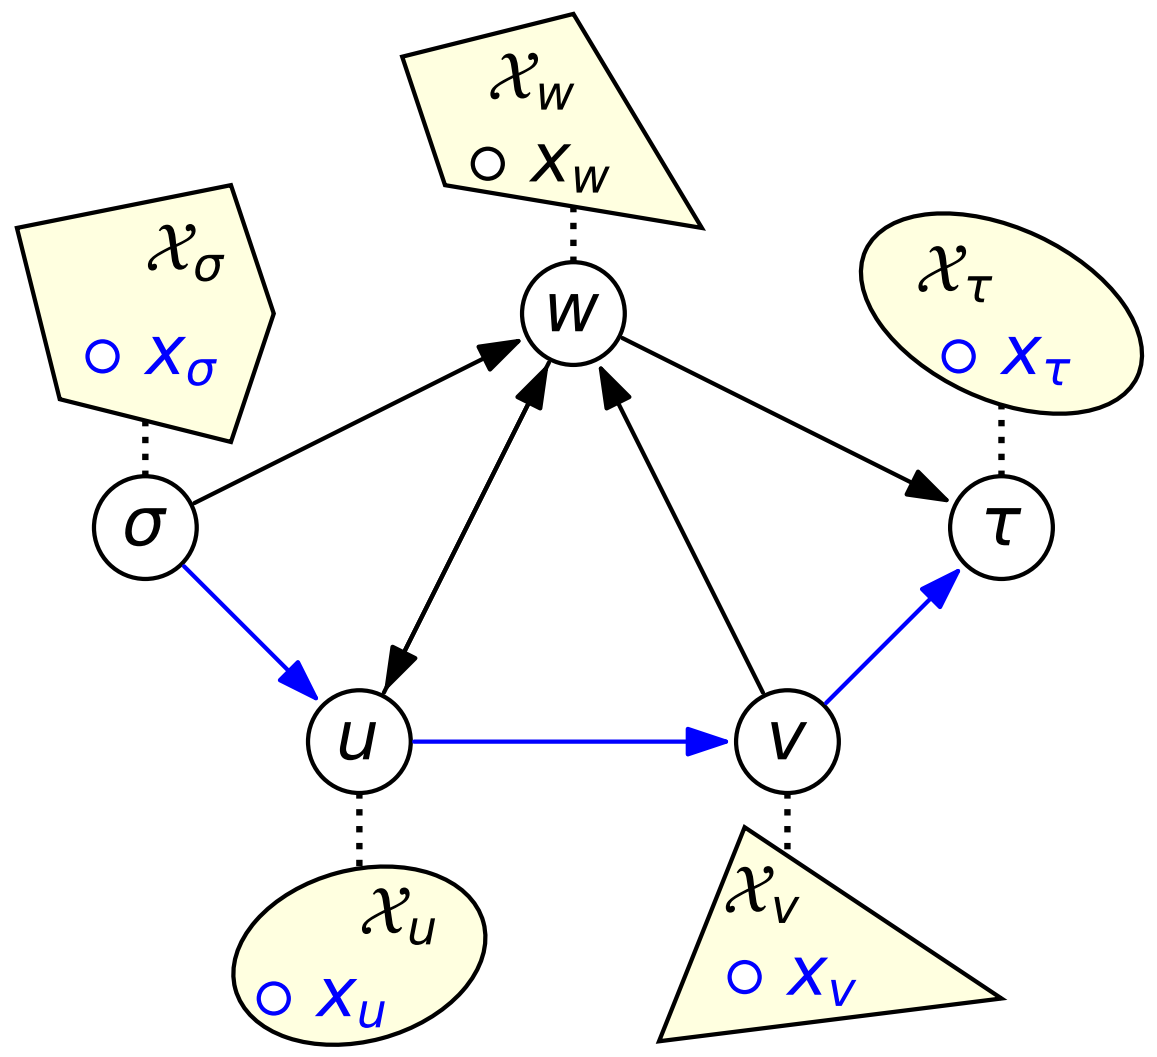
\includegraphics[width=0.8\linewidth]{./imgs/gcs-frame-2.png}
            \captionof{figure}{SPP trong GCS\footnotemark}
        \end{column}
    \end{columns}

    % \captionof{figure}{SPP in GCS\footnotemark}

    % \footnotetext{Nguồn: Shao Yuan et al., ``GCS*: Forward Heuristic Search on Implicit Graphs of Convex Sets''}
    \footnotetext{Nguồn: Marcucci et al., ``Motion Planning around Obstacles with Convex Optimization''}

\end{frame}

\begin{frame}{Hoạch định chuyển động}
    \textbf{Mô hình hóa bài toán:}
    % \vspace{0.1cm}
    \begin{equation*}
        \min_{q, T} \underbrace{aT}_{\text{Thời gian}} + \underbrace{b \int_{0}^{T} \|\dot{q}(t)\|_2 dt}_{\text{Độ dài}} + \underbrace{c \int_{0}^{T} \|\dot{q}(t)\|_2^2 dt}_{\text{Năng lượng}}
    \end{equation*}
    % \vspace{-0.2cm}
    \begin{itemize}
        \item \textbf{An toàn:} $q(t) \in \bigcup_{i \in \mathcal{I}} \mathcal{Q}_i$ (phân hoạch lồi)
        \item \textbf{Vật lý:} $\dot{q}(t) \in \mathcal{D}$ (tập vận tốc lồi), $q \in \mathcal{C}^\eta$ (trơn)
        \item \textbf{Ràng buộc biên:} $q(0) = q_{init}, \dot{q}(0) = v_{init}$; $q(T) = q_{final}, \dot{q}(T) = v_{final}$
              % \item \textbf{Lồi hóa:} hàm phối cảnh xử lý $T$ như biến quyết định
    \end{itemize}

    % \vspace{1em}
    % Cấu trúc lại qua tọa độ đường $s \in [0, 1]$: $q(t) = r(s)$ với $t = h(s)$
    % \begin{equation*}
    %     r(s) = \sum_{k=0}^{d} \beta_{k,d}(s)r_k, \quad h(s) = \sum_{k=0}^{d} \beta_{k,d}(s)h_k
    % \end{equation*}
\end{frame}

\begin{frame}{Hoạch định chuyển động sử dụng mô hình SPP trong GCS}
    \begin{columns}[T,onlytextwidth]
        \begin{column}{0.55\textwidth}
            Mục tiêu: Tìm quỹ đạo tối ưu $\sigma \to \tau$ trên GCS
            \begin{itemize}
                \item Phân hoạch không gian thành các vùng an toàn lồi $\{Q_v \subset R^2\}$
                \item Thiết lập đồ thị liền kề GCS $G=(V,\mathcal{E})$
                \item Gán biến trạng thái $x_v \in \mathcal{X}_v$ cho mọi $v \in V$:
                      \begin{itemize}
                          \item $x_v = (q_v^{s,x}, q_v^{s,y}, q_v^{m,x}, q_v^{m,y}, q_v^{t,x}, q_v^{t,y}) \in \mathbb{R}^6$
                          \item $\mathcal{X}_v = \{x_v \mid q_v^s, q_v^m, q_v^t \in Q_v\}$
                          \item Tại $s$ và $t$: $\mathcal{X}_{\sigma} := \mathcal{X}_{\tau} := \emptyset$
                      \end{itemize}

            \end{itemize}
        \end{column}
        \begin{column}{0.45\textwidth}
            \centering
            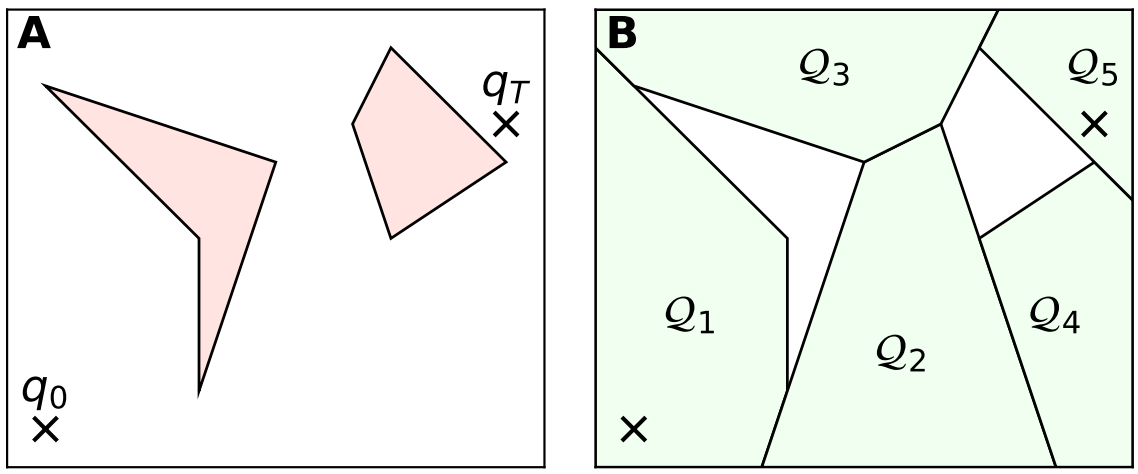
\includegraphics[width=\linewidth]{./imgs/gcs-1.png}
            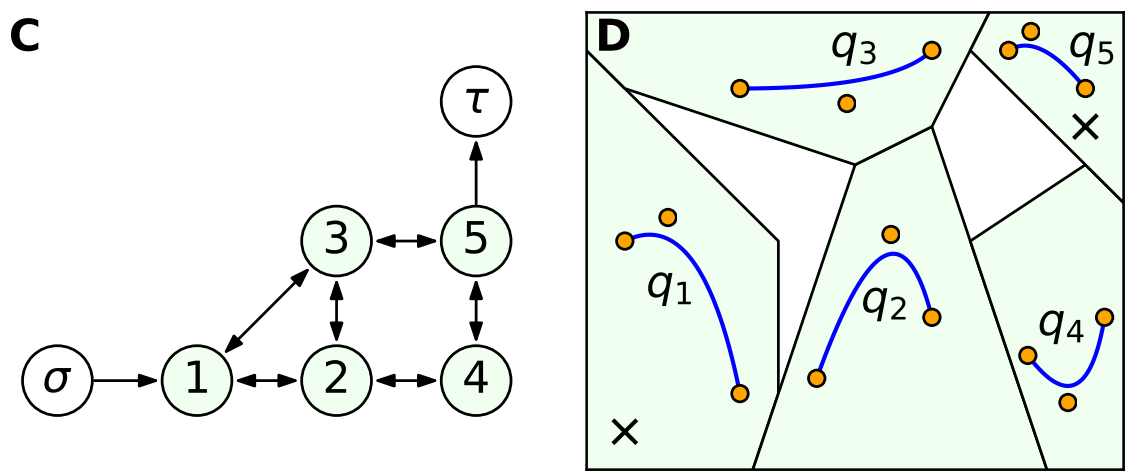
\includegraphics[width=\linewidth]{./imgs/gcs-2.png}
            \captionof{figure}{GCS Framework\footnotemark}
            % 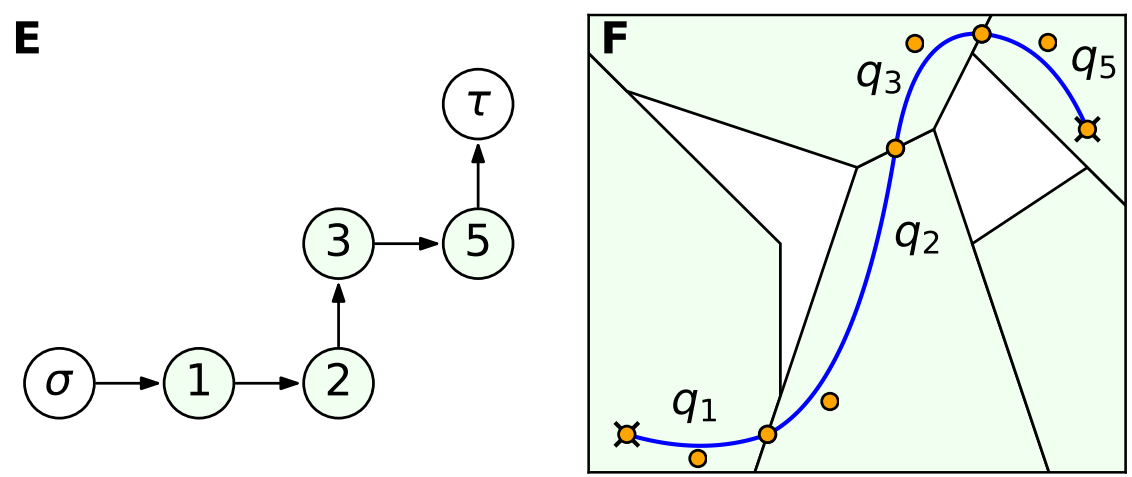
\includegraphics[width=0.7\linewidth]{./imgs/gcs-3.png}
        \end{column}
    \end{columns}

    \footnotetext{Nguồn: Marcucci et al., ``Motion Planning around Obstacles with Convex Optimization''}
\end{frame}

% \section{Kỹ thuật Convex Relaxation}
\begin{frame}{Hoạch định chuyển động sử dụng mô hình SPP trong GCS}

    \begin{columns}[T,onlytextwidth]
        \begin{column}{0.55\textwidth}
            \begin{itemize}
                \item Ràng buộc cạnh $\mathcal{X}_e$:
                      \begin{equation*}
                          \mathcal{X}_e = \left\{ (x_v, x_u) \middle|
                          \begin{aligned}
                              q_v^t         & = q_u^s         &  & \text{\small($C^0$)} \\
                              q_v^t - q_v^m & = q_u^m - q_u^s &  & \text{\small($C^1$)}
                          \end{aligned}
                          \right\}
                      \end{equation*}
                \item Hàm chi phí cạnh lồi, đóng $\ell_e$:
                      \begin{equation*}
                          \ell_e(x_u, x_v) = \int_0^{T_e} \|\dot{q}_e(t)\|^2 dt
                      \end{equation*}
            \end{itemize}

        \end{column}
        \begin{column}{0.45\textwidth}
            \centering
            % 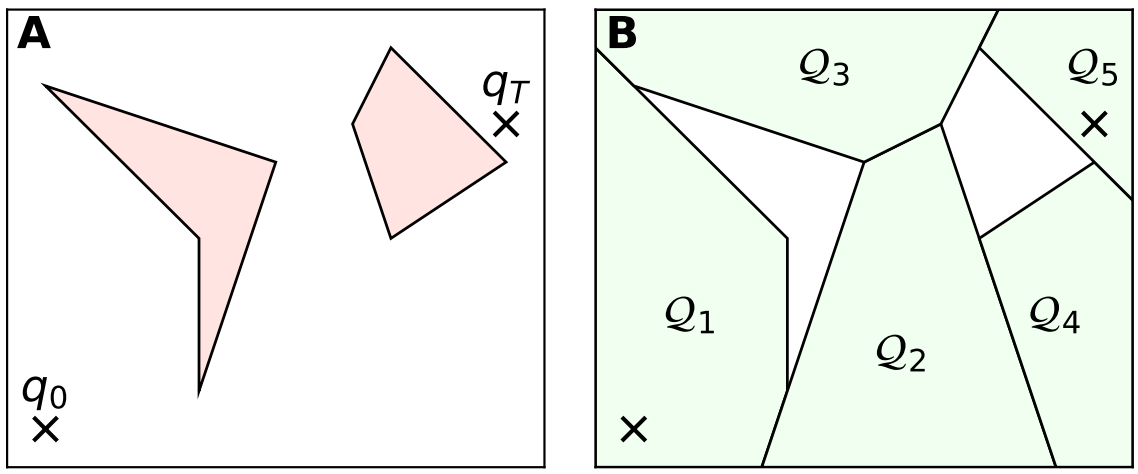
\includegraphics[width=0.7\linewidth]{./imgs/gcs-1.png}
            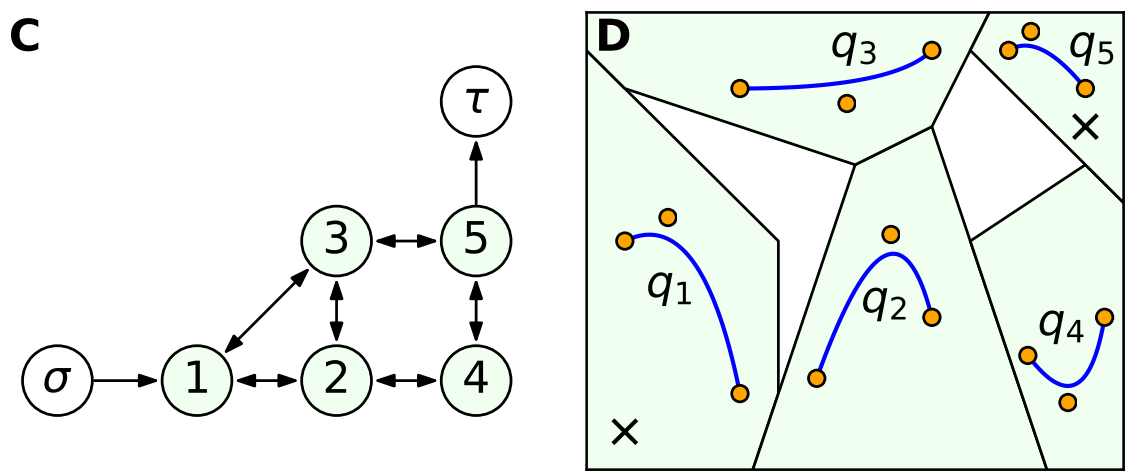
\includegraphics[width=\linewidth]{./imgs/gcs-2.png}
            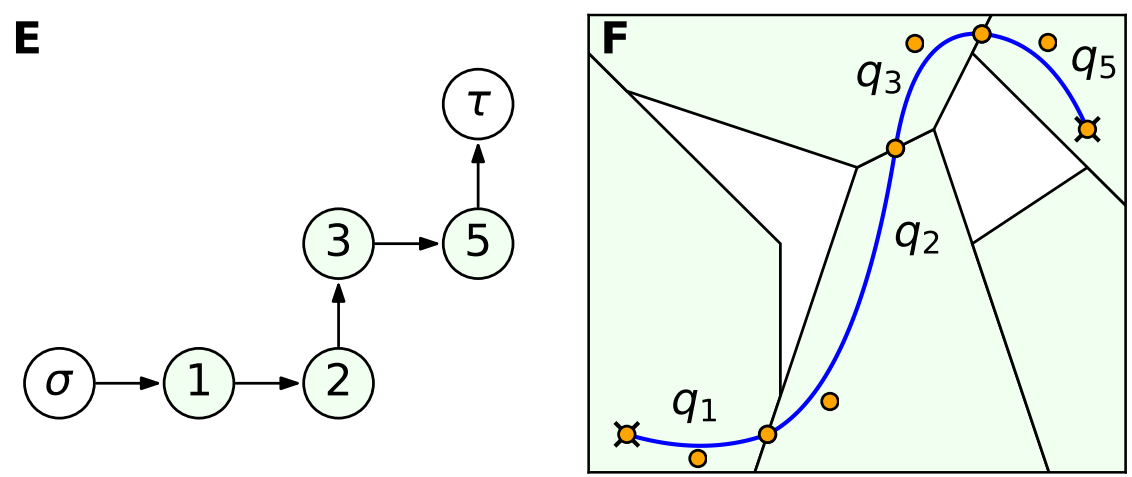
\includegraphics[width=\linewidth]{./imgs/gcs-3.png}
            \captionof{figure}{GCS Framework\footnotemark}
        \end{column}

    \end{columns}

    \footnotetext{Nguồn: Marcucci et al., ``Motion Planning around Obstacles with Convex Optimization''}
\end{frame}

% \begin{frame}{Đặc tính NP-hard và Nới lỏng Lồi}
%     \textbf{Bài toán:}
%     \begin{align}
%         \text{minimize} \quad   & \sum_{e=(u,v) \in
%         \mathcal{E}} y_e \ell_e(x_u, x_v) \label{eq:gcs_obj_milp}                                                                                                                \\
%         \text{subject to} \quad & \sum_{e \in \mathcal{E}^+(u)} y_e - \sum_{e \in \mathcal{E}^-(u)} y_e = \delta_u, \quad \forall u \in \mathcal{V} \label{eq:flow_conservation} \\
%                                 & (x_u, x_v) \in X_e, \quad \forall e=(u,v) \in \mathcal{E} \label{eq:edge_constraint}                                                           \\
%                                 & x_v \in X_v, \quad \forall v \in \mathcal{V} \label{eq:vertex_constraint}                                                                      \\
%                                 & y_e \in \{0, 1\}, \quad \forall e \in \mathcal{E} \label{eq:binary_variable}
%     \end{align}

%     \begin{itemize}
%         \item Lập trình hỗn hợp nguyên lồi (Mixed-Integer Convex Program - MICP),
%               NP-hard~\cite{marcucci2023motion}
%         \item \textbf{Giải pháp:} Nới lỏng $\rightarrow$ bài toán lồi chặt~\cite{marcucci2023motion,marcucci2024shortest}
%     \end{itemize}

% \end{frame}

% % \section{Phương pháp Rounding}
% \begin{frame}{Nới lỏng lồi (Convex Relaxation) và Giải thuật Làm tròn}
%     \textbf{Chiến lược nới lỏng bài toán MICP:}
%     \begin{itemize}
%         \item Hàm chi phí phi lồi và ràng buộc rời rạc $\rightarrow$ lồi: kỹ thuật hàm phối
%               cảnh~\cite{marcucci2023motion,marcucci2024shortest}.
%         \item Ràng buộc phi lồi $\rightarrow$ hệ ràng buộc lồi chặt $\Rightarrow$ tối ưu
%               lồi~\cite{marcucci2023motion,marcucci2024shortest}.
%     \end{itemize}
%     \textbf{Kết quả nới lỏng:}
%     \begin{itemize}
%         \item Kết quả cho ra thường chặt: $C_{relax} \approx C_{opt}$
%         \item Nếu không chặt (Loose Relaxation): làm tròn ngẫu nhiên
%         \item \textbf{Đánh giá:}
%               \begin{itemize}
%                   \item Khoảng cách tối ưu: $\delta_{opt} = \frac{C_{round} - C_{opt}}{C_{opt}}$
%                   \item Ước lượng qua nới lỏng: $\delta_{relax} = \frac{C_{round} - C_{relax}}{C_{relax}}$
%               \end{itemize}
%     \end{itemize}

%     \textbf{Làm tròn ngẫu nhiên:}
%     \begin{enumerate}
%         \item Khởi tạo từ nguồn $\sigma$
%         \item Tại nút $v$: chọn cạnh $e=(v \to w)$ theo xác suất $\propto y_e^*$
%         \item Quay lui nếu ngõ cụt, đến đích $\tau$~\cite{marcucci2023motion}
%     \end{enumerate}
% \end{frame}

% \begin{frame}{Sinh quỹ đạo liên tục}
%     \textbf{Sau khi chọn được đường đi rời rạc $p$:}
%     \begin{enumerate}
%         \item Cố định các biến nhị phân: $y_e = 1$ nếu $e \in p$, ngược lại $y_e = 0$
%         \item Giải bài toán lồi thuần túy với biến liên tục $x_v$
%         \item Bài toán rút gọn có quy mô rất nhỏ ("tiny convex program")
%         \item Giải rất nhanh nhờ cấu trúc đặc biệt \cite{marcucci2023motion}
%     \end{enumerate}

%     \vspace{0.5em}

%     \textbf{Kết quả:}
%     \begin{itemize}
%         \item Quỹ đạo tối ưu cho đường đi $p$ đã chọn
%         \item Thỏa mãn mọi ràng buộc: va chạm, liên tục, động học
%         \item Trơn tru nhờ tham số hóa Bézier với ràng buộc đạo hàm \cite{marcucci2023motion}
%     \end{itemize}
% \end{frame}

% \section{So sánh với phương pháp Sampling-based}

% \begin{frame}{Ưu điểm của GCS}
% \begin{multicols}{2}
%     \textbf{1. Tối ưu toàn cục}

%     \textbf{2. Ràng buộc động học}
%     \begin{itemize}
%         \item GCS: tích hợp trực tiếp
%         \item PRM/RRT: cần hậu xử lý
%     \end{itemize}

%     \columnbreak

%     \textbf{3. Tính đầy đủ}
%     \begin{itemize}
%         \item GCS: chứng nhận khả thi/không khả thi
%         \item PRM/RRT: không chắc chắn \cite{marcucci2023motion}
%     \end{itemize}

%     \textbf{4. Không gian hẹp}
% \end{multicols}
% \end{frame}

\section{Thực nghiệm}

% =====================================================================
% Slide 1: Setup overview
% =====================================================================
\begin{frame}{Thiết lập thực nghiệm}
\vspace{-0.6em}

{\scriptsize\color{black!65}
Hai formulation được chạy trong cùng cấu hình; mỗi thực nghiệm kiểm tra một khía cạnh riêng của bài toán.
}

\vspace{0.35em}

\begin{columns}[T,onlytextwidth]
% ================= LEFT =================
\begin{column}{0.55\textwidth}
\begin{block}{Stack triển khai}
\vspace{-0.55em}
\scriptsize
\centering
\setlength{\tabcolsep}{3.5pt}
\renewcommand{\arraystretch}{1.12}

\begin{tabular}{@{}lll@{}}
\toprule
\textbf{Pha} &
\textbf{\textcolor{blue!75!black}{GCS-Bézier}} &
\textbf{\textcolor{teal!70!black}{GCS-DMS}} \\
\midrule
Phân hoạch & \multicolumn{2}{c}{ACD / IRIS / VCC (Drake)} \\
Solver     & Mosek (SOCP)   & CasADi + IPOPT (NLP) \\
Ngôn ngữ   & Python (Drake) & Python \\
\bottomrule
\end{tabular}

\vspace{0.35em}
{\tiny
\textbf{Phần cứng:} AMD Ryzen 7 4800H @ 2.9 GHz; 16 GB RAM; Ubuntu 24.04.
}
\end{block}
\end{column}

% ================= RIGHT =================
\begin{column}{0.43\textwidth}
\vspace{-0.55em}
\centering
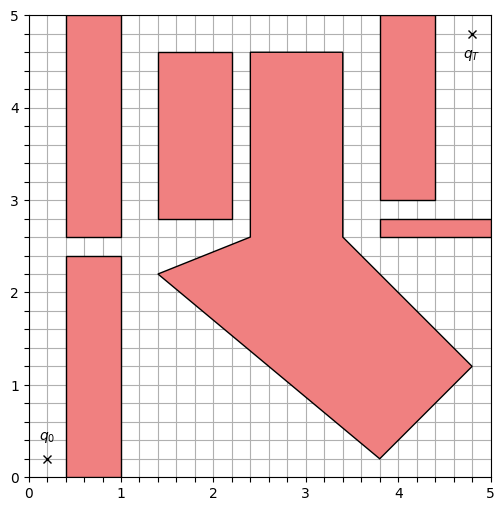
\includegraphics[
    width=0.6\linewidth,
    % height=0.26\textheight,
    keepaspectratio
]{./imgs/2d-env.png}
\end{column}
\end{columns}

\vspace{-0.25em}

\begin{beamercolorbox}[wd=\textwidth,sep=1.5pt,rounded=true]{block title example}
{\footnotesize\textbf{Thực nghiệm:}}
\end{beamercolorbox}

\vspace{0.25em}

\begin{columns}[T,onlytextwidth]
% ================= CARD 1 =================
\begin{column}{0.32\textwidth}
\centering
\begin{tikzpicture}
\node[
    fill=teal!8,
    draw=teal!45,
    rounded corners=2pt,
    inner sep=3pt,
    minimum height=1.05cm,
    text width=0.92\linewidth,
    align=left
] {
{\scriptsize\textbf{\textcolor{teal!70!black}{TN3 -- 2D đơn giản}}}\\[-0.15em]
{\tiny Manual / ACD / VCC}\\[-0.15em]
{\tiny Tác động của thuật toán phân hoạch.}
};
\end{tikzpicture}
\end{column}

% ================= CARD 2 =================
\begin{column}{0.32\textwidth}
\centering
\begin{tikzpicture}
\node[
    fill=blue!8,
    draw=blue!45,
    rounded corners=2pt,
    inner sep=3pt,
    minimum height=1.05cm,
    text width=0.92\linewidth,
    align=left
] {
{\scriptsize\textbf{\textcolor{blue!75!black}{TN2 -- Maze $25\!\times\!25$}}}\\[-0.15em]
{\tiny 10 mẫu ngẫu nhiên}\\[-0.15em]
{\tiny Mở rộng tổ hợp của GCS-Bézier.}
};
\end{tikzpicture}
\end{column}

% ================= CARD 3 =================
\begin{column}{0.32\textwidth}
\centering
\begin{tikzpicture}
\node[
    fill=red!6!yellow!8,
    draw=red!55!yellow!45,
    rounded corners=2pt,
    inner sep=3pt,
    minimum height=1.05cm,
    text width=0.92\linewidth,
    align=left
] {
{\scriptsize\textbf{\textcolor{red!65!yellow!45!black}{TN1 -- Unicycle}}}\\[-0.15em]
{\tiny 2D + maze $15\!\times\!15$}\\[-0.15em]
{\tiny GCS-DMS với động lực học phi tuyến.}
};
\end{tikzpicture}
\end{column}
\end{columns}

\end{frame}
% =====================================================================
% Slide 2: Evaluation metrics
% =====================================================================
\begin{frame}{Chỉ số đánh giá}
\vspace{-0.45em}

{\scriptsize\color{black!65}
Hai formulation giải hai bài toán khác nhau $\Rightarrow$ chỉ số dùng để
\textbf{kiểm chứng từng mô hình}, không xếp hạng trực tiếp.
}

\vspace{0.45em}

\begin{columns}[T,onlytextwidth]

% ================= COL 1 =================
\begin{column}{0.32\textwidth}
\begin{block}{Chi phí tính toán}

\scriptsize
\begin{itemize}
    \setlength\itemsep{0.22em}
    \item $t_{\text{decomp}}$: thời gian phân hoạch
    \item $t_{\text{solve}}$: thời gian giải tối ưu
    \item $N_{\text{region}}$: số vùng toàn cục / kích hoạt
\end{itemize}
\vspace{-0.35em}
\end{block}
\end{column}

% ================= COL 2 =================
\begin{column}{0.32\textwidth}
\begin{exampleblock}{Chất lượng quỹ đạo}

\scriptsize
\begin{itemize}
    \setlength\itemsep{0.22em}
    \item $T_{\text{exec}}$: thời gian thực thi
    \item $C_{\text{path}}$ / $C_{\text{DMS}}$: giá trị mục tiêu
    \item $|v(t)|$: hồ sơ vận tốc
\end{itemize}
\vspace{-0.35em}
\end{exampleblock}
\end{column}

% ================= COL 3 =================
\begin{column}{0.32\textwidth}
\begin{alertblock}{Tính khả thi}

\scriptsize
\begin{itemize}
    \setlength\itemsep{0.22em}
    \item Optimality gap của GCS-Bézier
    \item Defect / connection gap của DMS
    \item Violation và integrality gap
\end{itemize}
\vspace{-0.35em}
\end{alertblock}
\end{column}

\end{columns}

\vspace{0.35em}

\begin{beamercolorbox}[
    wd=\textwidth,
    sep=3pt,
    rounded=true
]{block title example}
{\scriptsize
\textbf{Ghi chú:}
Một số chỉ số chỉ có nghĩa với một mô hình; chỉ số chung chỉ đóng vai trò mô tả.
}
\end{beamercolorbox}

\end{frame}

% =====================================================================
% TN3 - Slide 1: Decomposition visualization
% =====================================================================
\begin{frame}{TN3 — Ba phương pháp phân hoạch lồi (đầu vào)}
    \centering
    {\footnotesize Cùng môi trường 2D, cùng $q_0/q_T$, khác chiến lược phân hoạch.}

    \vspace{0.4em}
    \begin{minipage}{0.32\linewidth}
        \centering
        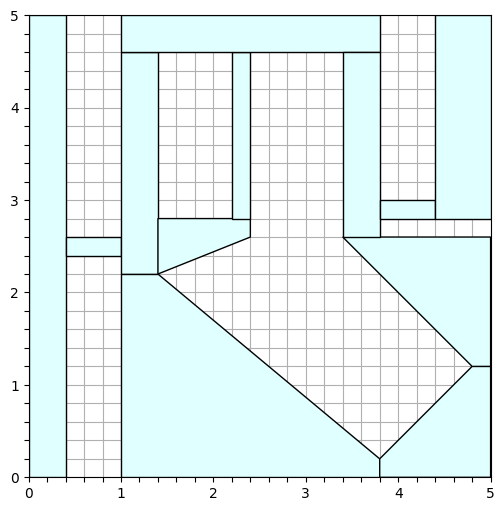
\includegraphics[height=3.6cm]{./imgs/manual_decompose.png}\\
        \textbf{Manual} \,---\, 12 vùng\\
        {\scriptsize $t_{\text{decomp}}$ không tính}
    \end{minipage}\hfill
    \begin{minipage}{0.32\linewidth}
        \centering
        \includegraphics[height=3.6cm]{./imgs/acd_decompose.png}\\
        \textbf{ACD} \,---\, 15 vùng\\
        {\scriptsize $\tau=0$; $t_{\text{decomp}}=0.01$ s}
    \end{minipage}\hfill
    \begin{minipage}{0.32\linewidth}
        \centering
        \includegraphics[height=3.6cm]{./imgs/vcc_decompose.png}\\
        \textbf{VCC} \,---\, $\sim$33 vùng\\
        {\scriptsize Phủ 96\%; $t_{\text{decomp}}=5.78$ s}
    \end{minipage}

    % \vspace{0.5em}
    \begin{exampleblock}{Quan sát}
        \footnotesize ACD bám sát mức tối thiểu của Manual với chi phí tự động hóa thấp; VCC tạo cấu trúc dày đặc hơn $\Rightarrow$ đồ thị GCS nhiều cạnh hơn.
    \end{exampleblock}
\end{frame}

% =====================================================================
% TN3 - Slide 2: GCS-Bezier trajectories + table
% =====================================================================
\begin{frame}{TN3 — Tác động lên GCS-Bézier}
    \begin{columns}[T,onlytextwidth]
        \begin{column}{0.46\textwidth}
            \centering
            \begin{minipage}{0.48\linewidth}
                \centering
                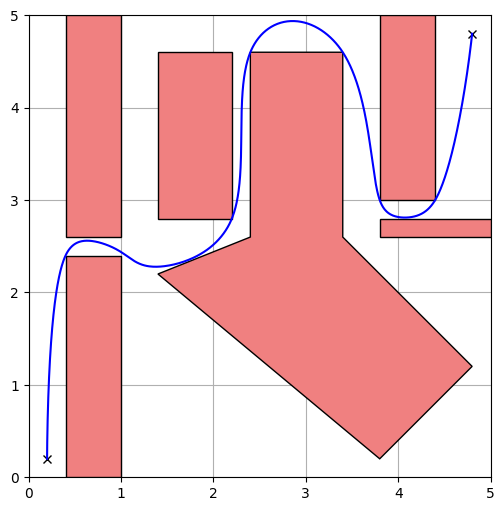
\includegraphics[height=2.6cm]{./imgs/manual_traj.png}\\
                {\scriptsize Manual}
            \end{minipage}\hfill
            \begin{minipage}{0.48\linewidth}
                \centering
                
\includegraphics[height=2.6cm]{./imgs/acd_traj.png}\\
                {\scriptsize ACD}
            \end{minipage}\\[0.3em]
            \begin{minipage}{0.5\linewidth}
                \centering
                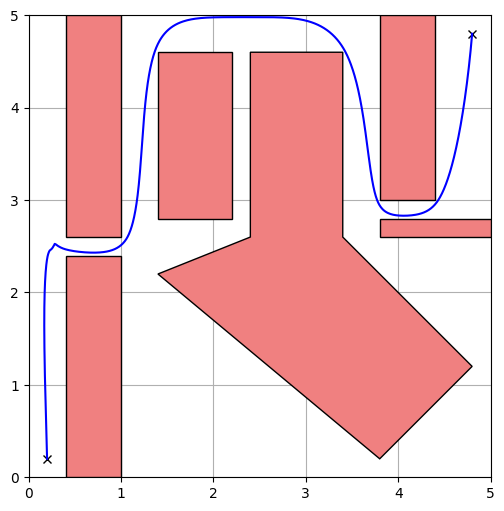
\includegraphics[height=2.6cm]{./imgs/VCC_traj.png}\\
                {\scriptsize VCC}
            \end{minipage}
        \end{column}
        \begin{column}{0.54\textwidth}
            \footnotesize
            \begin{table}
                \centering\footnotesize
                \begin{tabular}{lcccc}
                    \toprule
                    & \textbf{Vùng} & \textbf{Solve (s)} & \textbf{Path cost} & \textbf{Tổng (s)} \\
                    \midrule
                    Manual & 12 & \textbf{3.90}  & 27.88           & \textbf{3.90}   \\
                    ACD    & 15 & 4.31           & 24.63           & 4.32            \\
                    VCC    & 33 & 269.94         & \textbf{24.44}  & 275.72          \\
                    \bottomrule
                \end{tabular}
            \end{table}
            \vspace{-0.4em}
            \begin{alertblock}{Bài học}
                \scriptsize
                \begin{itemize}
                    \item \textbf{ACD cân bằng nhất:} tự động, $C_{\text{path}}$ gần VCC, nhanh hơn $\sim$64$\times$.
                    \item VCC: $t_{\text{solve}}$ \textbf{bùng nổ} do số biến nhị phân $\propto|\mathcal{E}|$ tăng phi tuyến.
                    \item Manual: nhanh nhưng \textit{không tự động} $\Rightarrow$ không khả thi cho rô-bốt tự hành.
                \end{itemize}
            \end{alertblock}
        \end{column}
    \end{columns}
\end{frame}

% =====================================================================
% TN3 - Slide 3: GCS-DMS on same decompositions
% =====================================================================
\begin{frame}{TN3 — Tác động lên GCS-DMS (Unicycle)}
\vspace{-0.55em}

\begin{columns}[T,onlytextwidth]

% ================= LEFT: FIGURES =================
\begin{column}{0.61\textwidth}
\centering

\begin{minipage}[t]{0.49\linewidth}
    \centering
    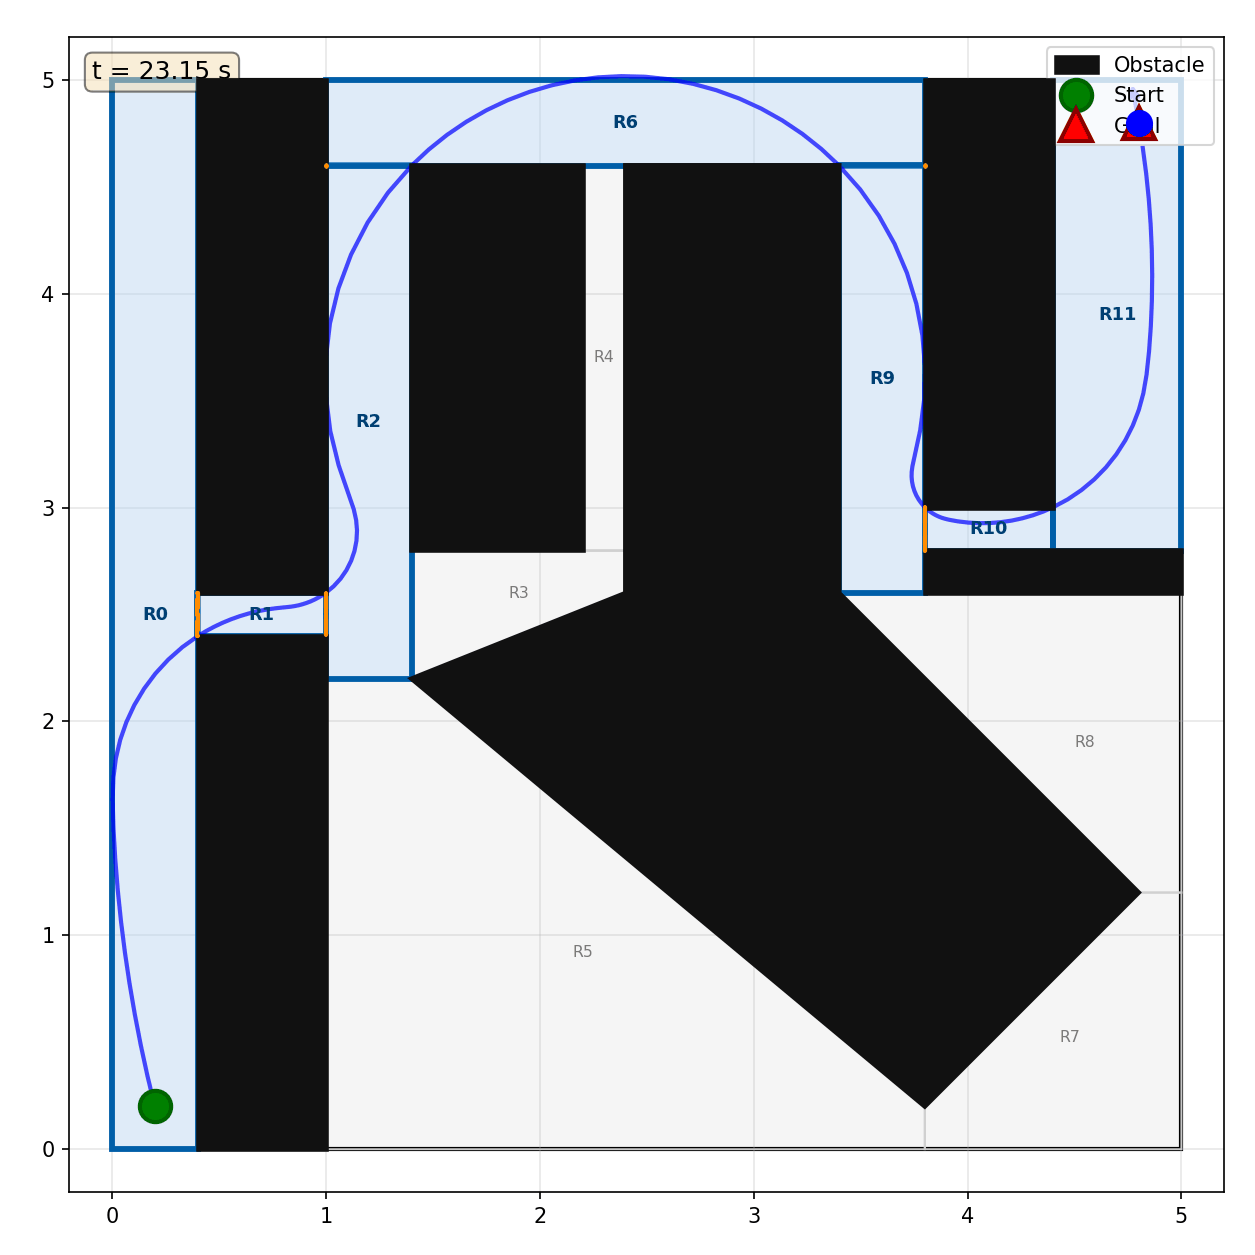
\includegraphics[
        height=3.5cm,
        keepaspectratio
    ]{./imgs/dms/2d_dms_manual.png}\\[-0.2em]
    {\tiny\bfseries Manual}
\end{minipage}
\hfill
\begin{minipage}[t]{0.49\linewidth}
    \centering
    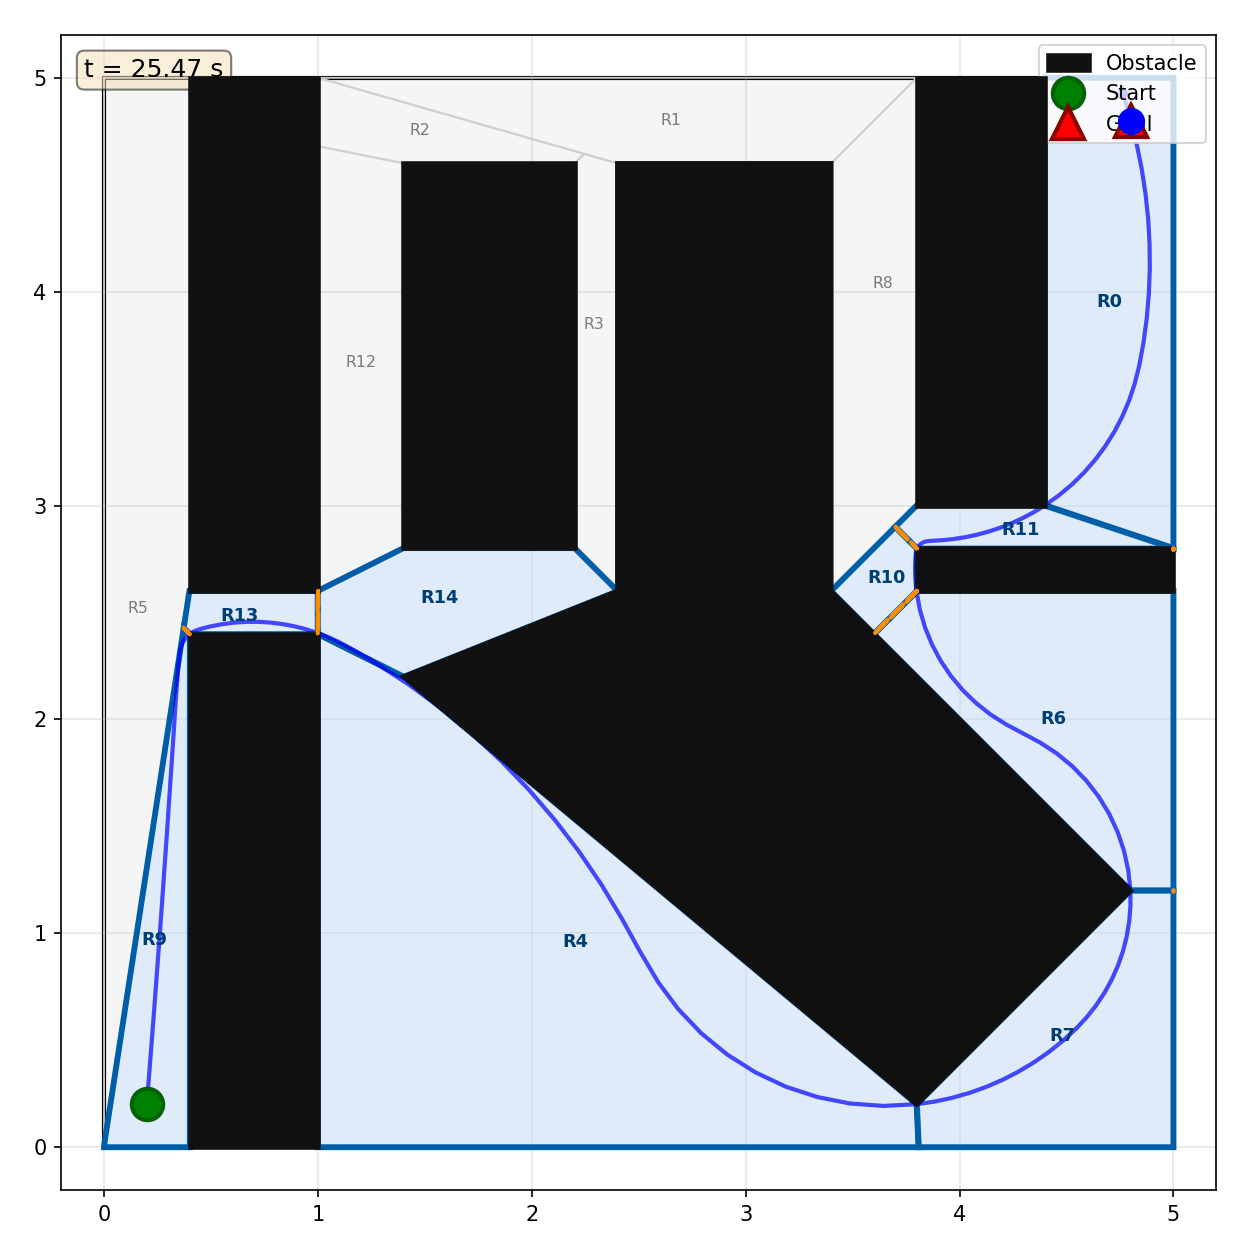
\includegraphics[
        height=3.5cm,
        keepaspectratio
    ]{./imgs/dms/2d_dms_acd.png}\\[-0.2em]
    {\tiny\bfseries ACD}
\end{minipage}

\vspace{0.05em}

\begin{minipage}[t]{0.58\linewidth}
    \centering
    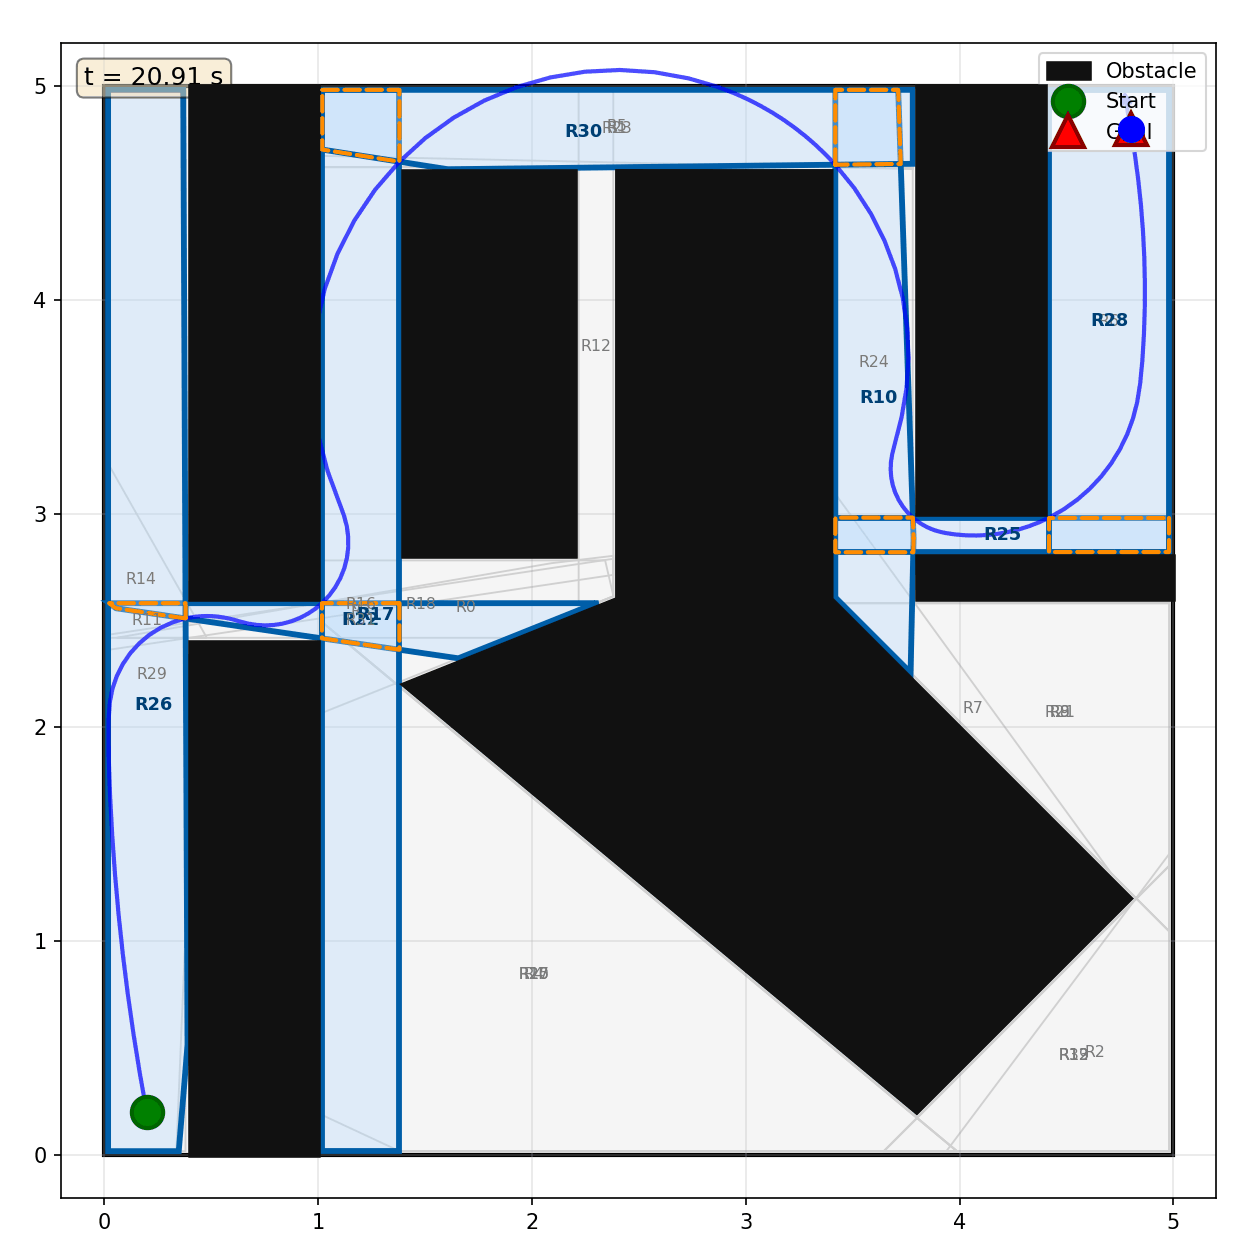
\includegraphics[
        height=3cm,
        keepaspectratio
    ]{./imgs/dms/2d_dms_vcc.png}\\[-0.2em]
    {\tiny\bfseries VCC}
\end{minipage}

\end{column}

% ================= RIGHT: TABLE + NOTE =================
\begin{column}{0.37\textwidth}
\vspace{0.25em}

\begin{block}{So sánh nghiệm}
\centering
\tiny
\setlength{\tabcolsep}{2.35pt}
\renewcommand{\arraystretch}{1.08}

\begin{tabular}{@{}lrrrr@{}}
\toprule
\textbf{PP} & \textbf{Vùng} & \textbf{K.hoạt} & \textbf{Cost} & \textbf{Solve} \\
\midrule
Manual & 12 & 7 & \textbf{47.35} & \textbf{17.38} \\
ACD    & 15 & 9 & 51.55          & 34.23          \\
VCC    & 33 & 7 & 76.26          & 26.36          \\
\bottomrule
\end{tabular}
\vspace{-0.55em}
\end{block}

\vspace{0.15em}

\begin{exampleblock}{Thông điệp chính}

\scriptsize
\begin{itemize}
    \setlength\itemsep{0.12em}
    \item Defect $\sim 10^{-14}$; gap $\sim 10^{-9}$; vi phạm $\sim 10^{-8}$.
    \item \textbf{Số vùng kích hoạt} quyết định chất lượng nghiệm DMS hơn số vùng toàn cục.
\end{itemize}
\vspace{-0.65em}
\end{exampleblock}

\end{column}

\end{columns}
\end{frame}

% =====================================================================
% TN2 - Combined slide: Maze 25x25
% =====================================================================
\begin{frame}{TN2 — Mê cung $25\!\times\!25$: Linear vs Bézier GCS}
    \begin{columns}[T,onlytextwidth]
        \begin{column}{0.55\textwidth}
            \centering
            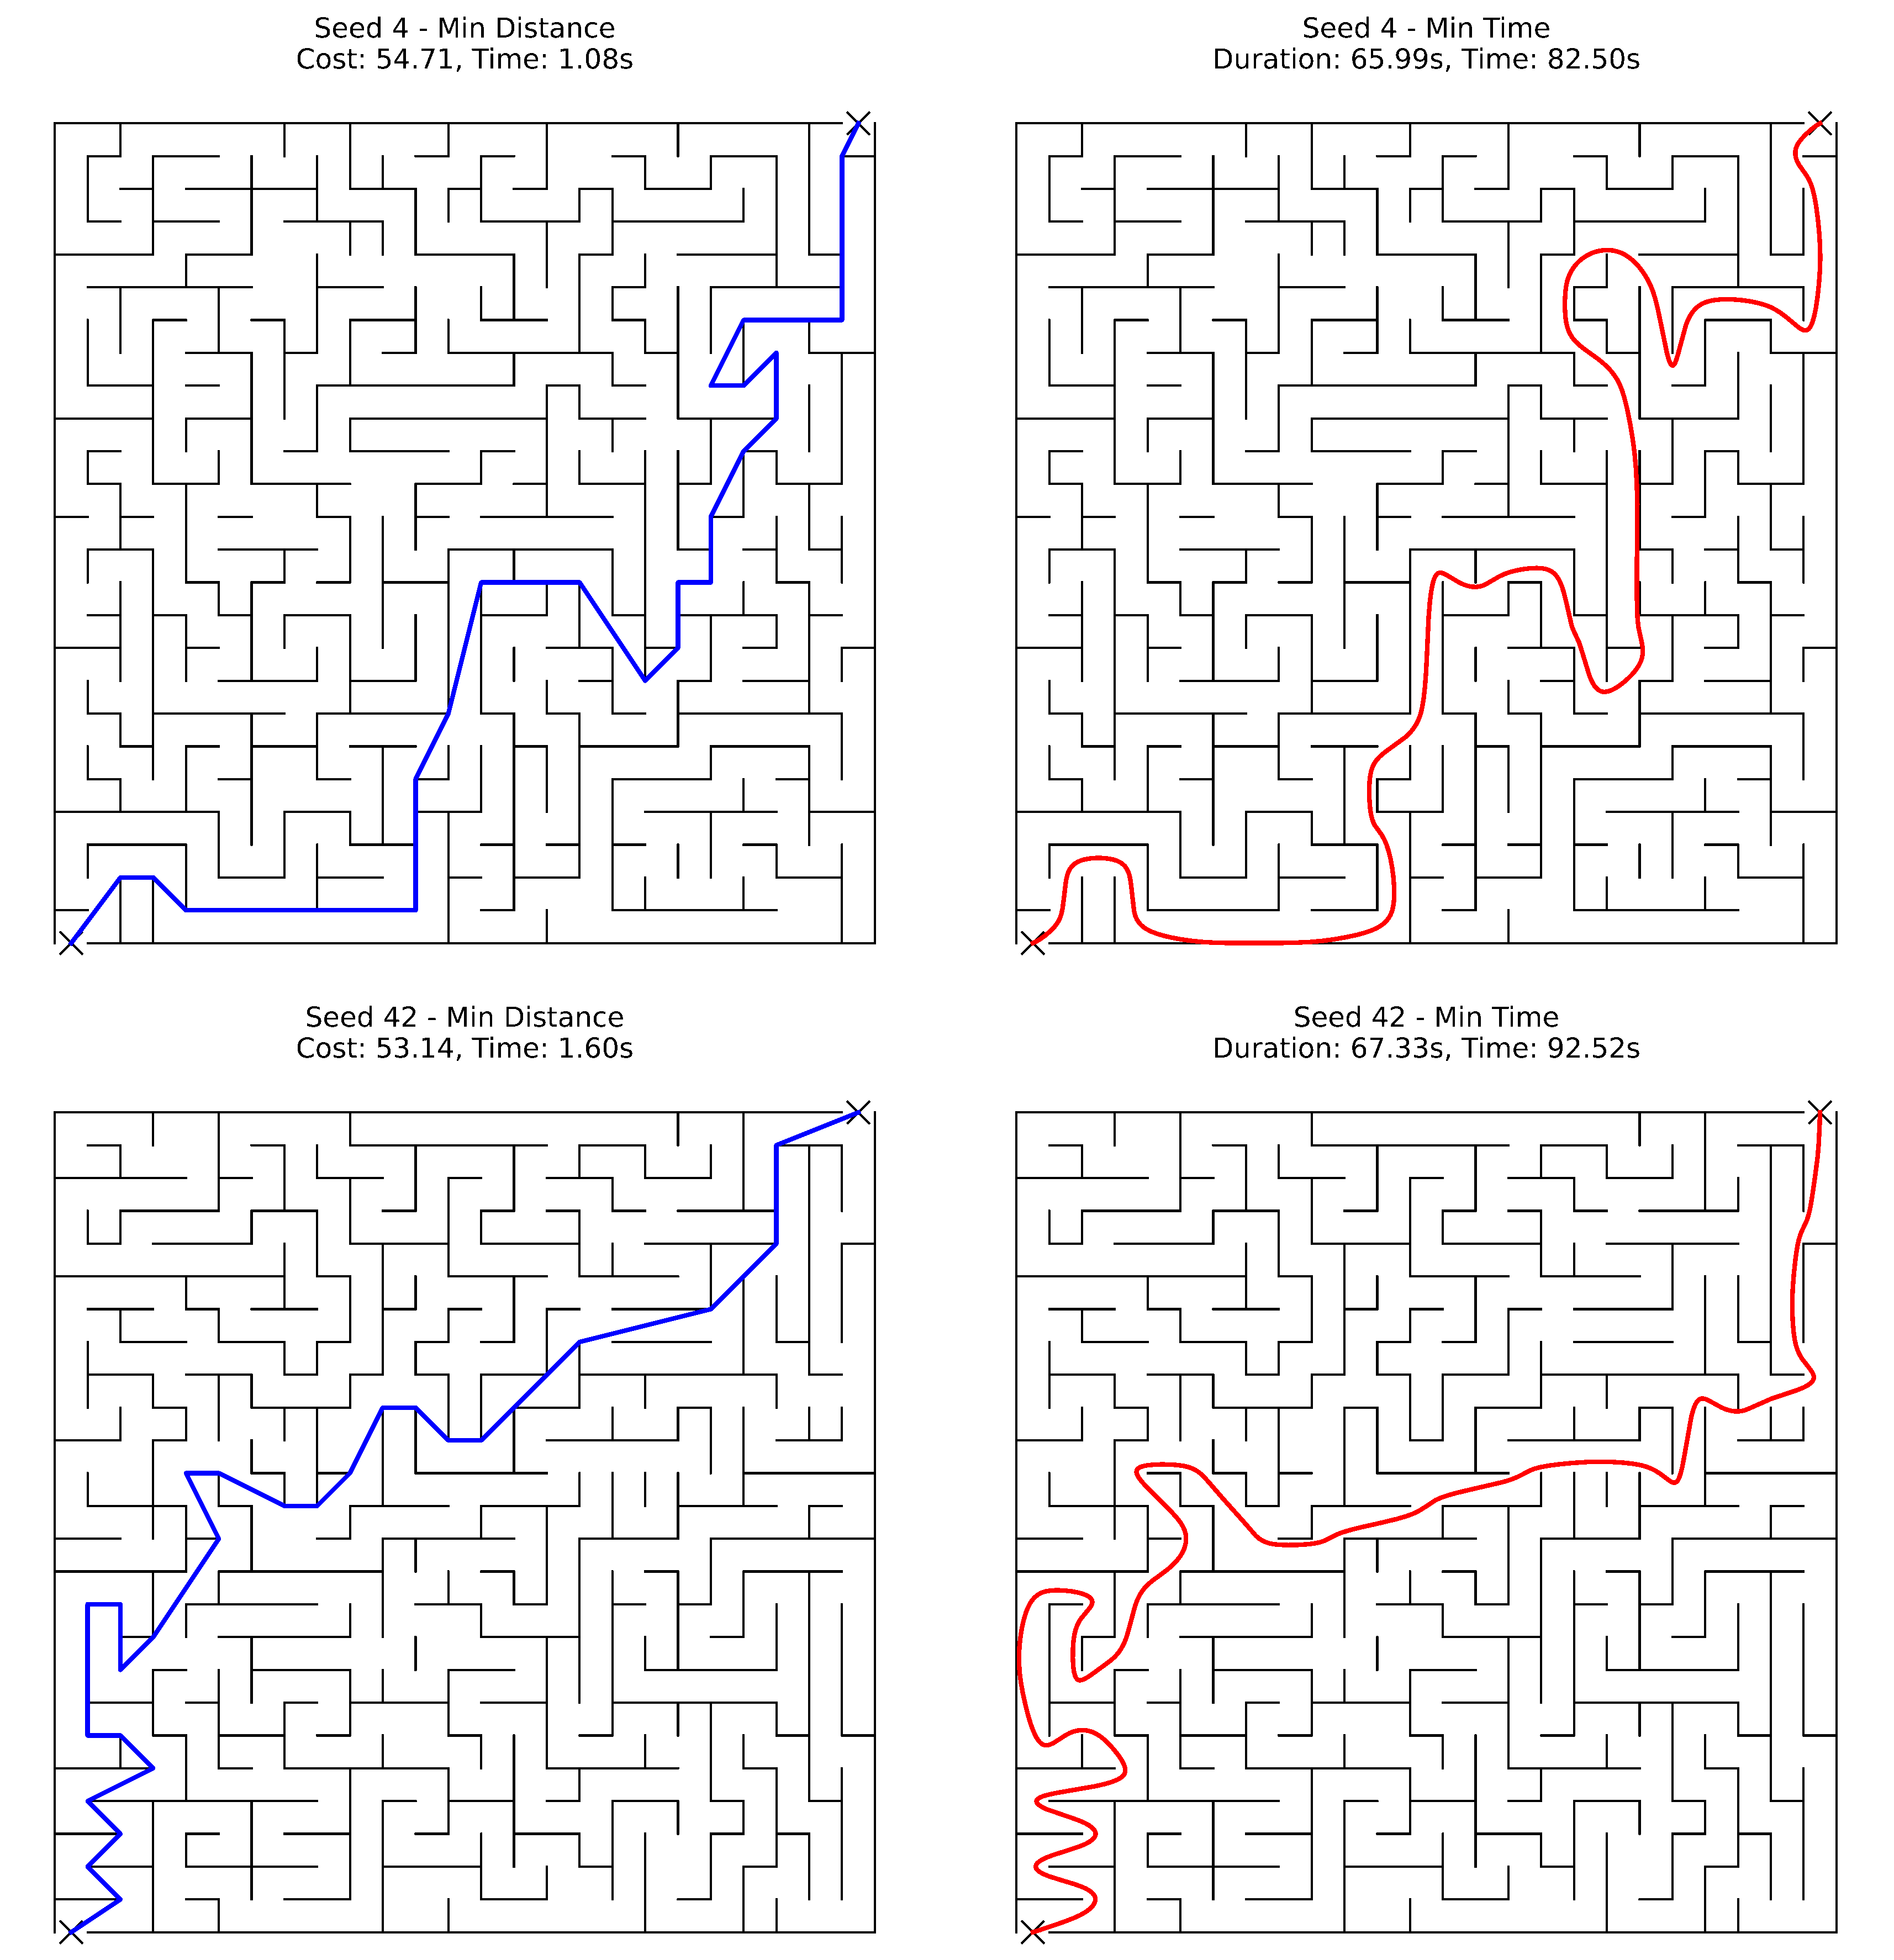
\includegraphics[width=0.7\textwidth]{./imgs/maze-1.png}\\[-0.2em]
            {\scriptsize Cùng homotopy: Bézier \textit{ôm cua rộng} để duy trì $C^2$}\\[0.3em]
        \end{column}
        \begin{column}{0.45\textwidth}
            \begin{block}{Thiết lập}
                \footnotesize 10 mê cung DFS ngẫu nhiên $25\!\times\!25\!=\!625$ ô, loại bỏ 100 tường. Bézier bậc $d=6$, $C^2$, $\dot{q}\in[-1,1]$.
            \end{block}
            \footnotesize
            \centering
            \begin{tabular}{lcc}
                \toprule
                \textbf{TB 10 mẫu} & \textbf{Linear} & \textbf{Bézier} \\
                \midrule
                Solve (s)   & \textbf{1.28}  & 85.22 \\
                Median (s)  & 1.16           & 85.10 \\
                Mean cost   & 71.88          & 88.03 \\
                Cost ratio  & 0.82           & 1.00  \\
                \bottomrule
            \end{tabular}
            \begin{exampleblock}{Tính tối ưu toàn cục}
                \scriptsize Trên \textbf{cả 10 mê cung}: $y_e^*\!\in\!\{0,1\}$ tự động $\Rightarrow$ \textbf{optimality gap $\boldsymbol{=0\%}$}, không cần rounding.
            \end{exampleblock}
        \end{column}
    \end{columns}
\end{frame}

% =====================================================================
% TN2 - Combinatorial scalability insight slide
% =====================================================================
\begin{frame}{TN2 — Vì sao GCS xử lý được 625 ô?}
    \begin{columns}[T,onlytextwidth]
        \begin{column}{0.55\textwidth}
            \begin{alertblock}{MICP truyền thống}
                \footnotesize
                Mỗi đoạn quỹ đạo cần biến nhị phân gán vào 1 trong $|I|$ vùng $\Rightarrow$ \textbf{$|I|^2$ biến nhị phân}.
                \vspace{0.3em}
                \[
                    625 \text{ ô} \;\Rightarrow\; |I|^2 = 390{,}625 \text{ biến}
                \]
                $\Rightarrow$ \textit{Không giải được trong thực tế.}
            \end{alertblock}
            \begin{exampleblock}{GCS (network flow)}
                \footnotesize
                Chỉ tạo biến nhị phân cho \textbf{cạnh giữa hai vùng kề}; bậc đồ thị 2D thấp $\Rightarrow$ \textbf{$|\mathcal{E}|\approx 2|I|$}.
                \vspace{0.3em}
                \[
                    625 \text{ ô} \;\Rightarrow\; 2|I| \approx 1{,}250 \text{ biến}
                \]
                $\Rightarrow$ \textit{Giải được trong $\sim$85 s.}
            \end{exampleblock}
        \end{column}
        \begin{column}{0.45\textwidth}
            \centering
            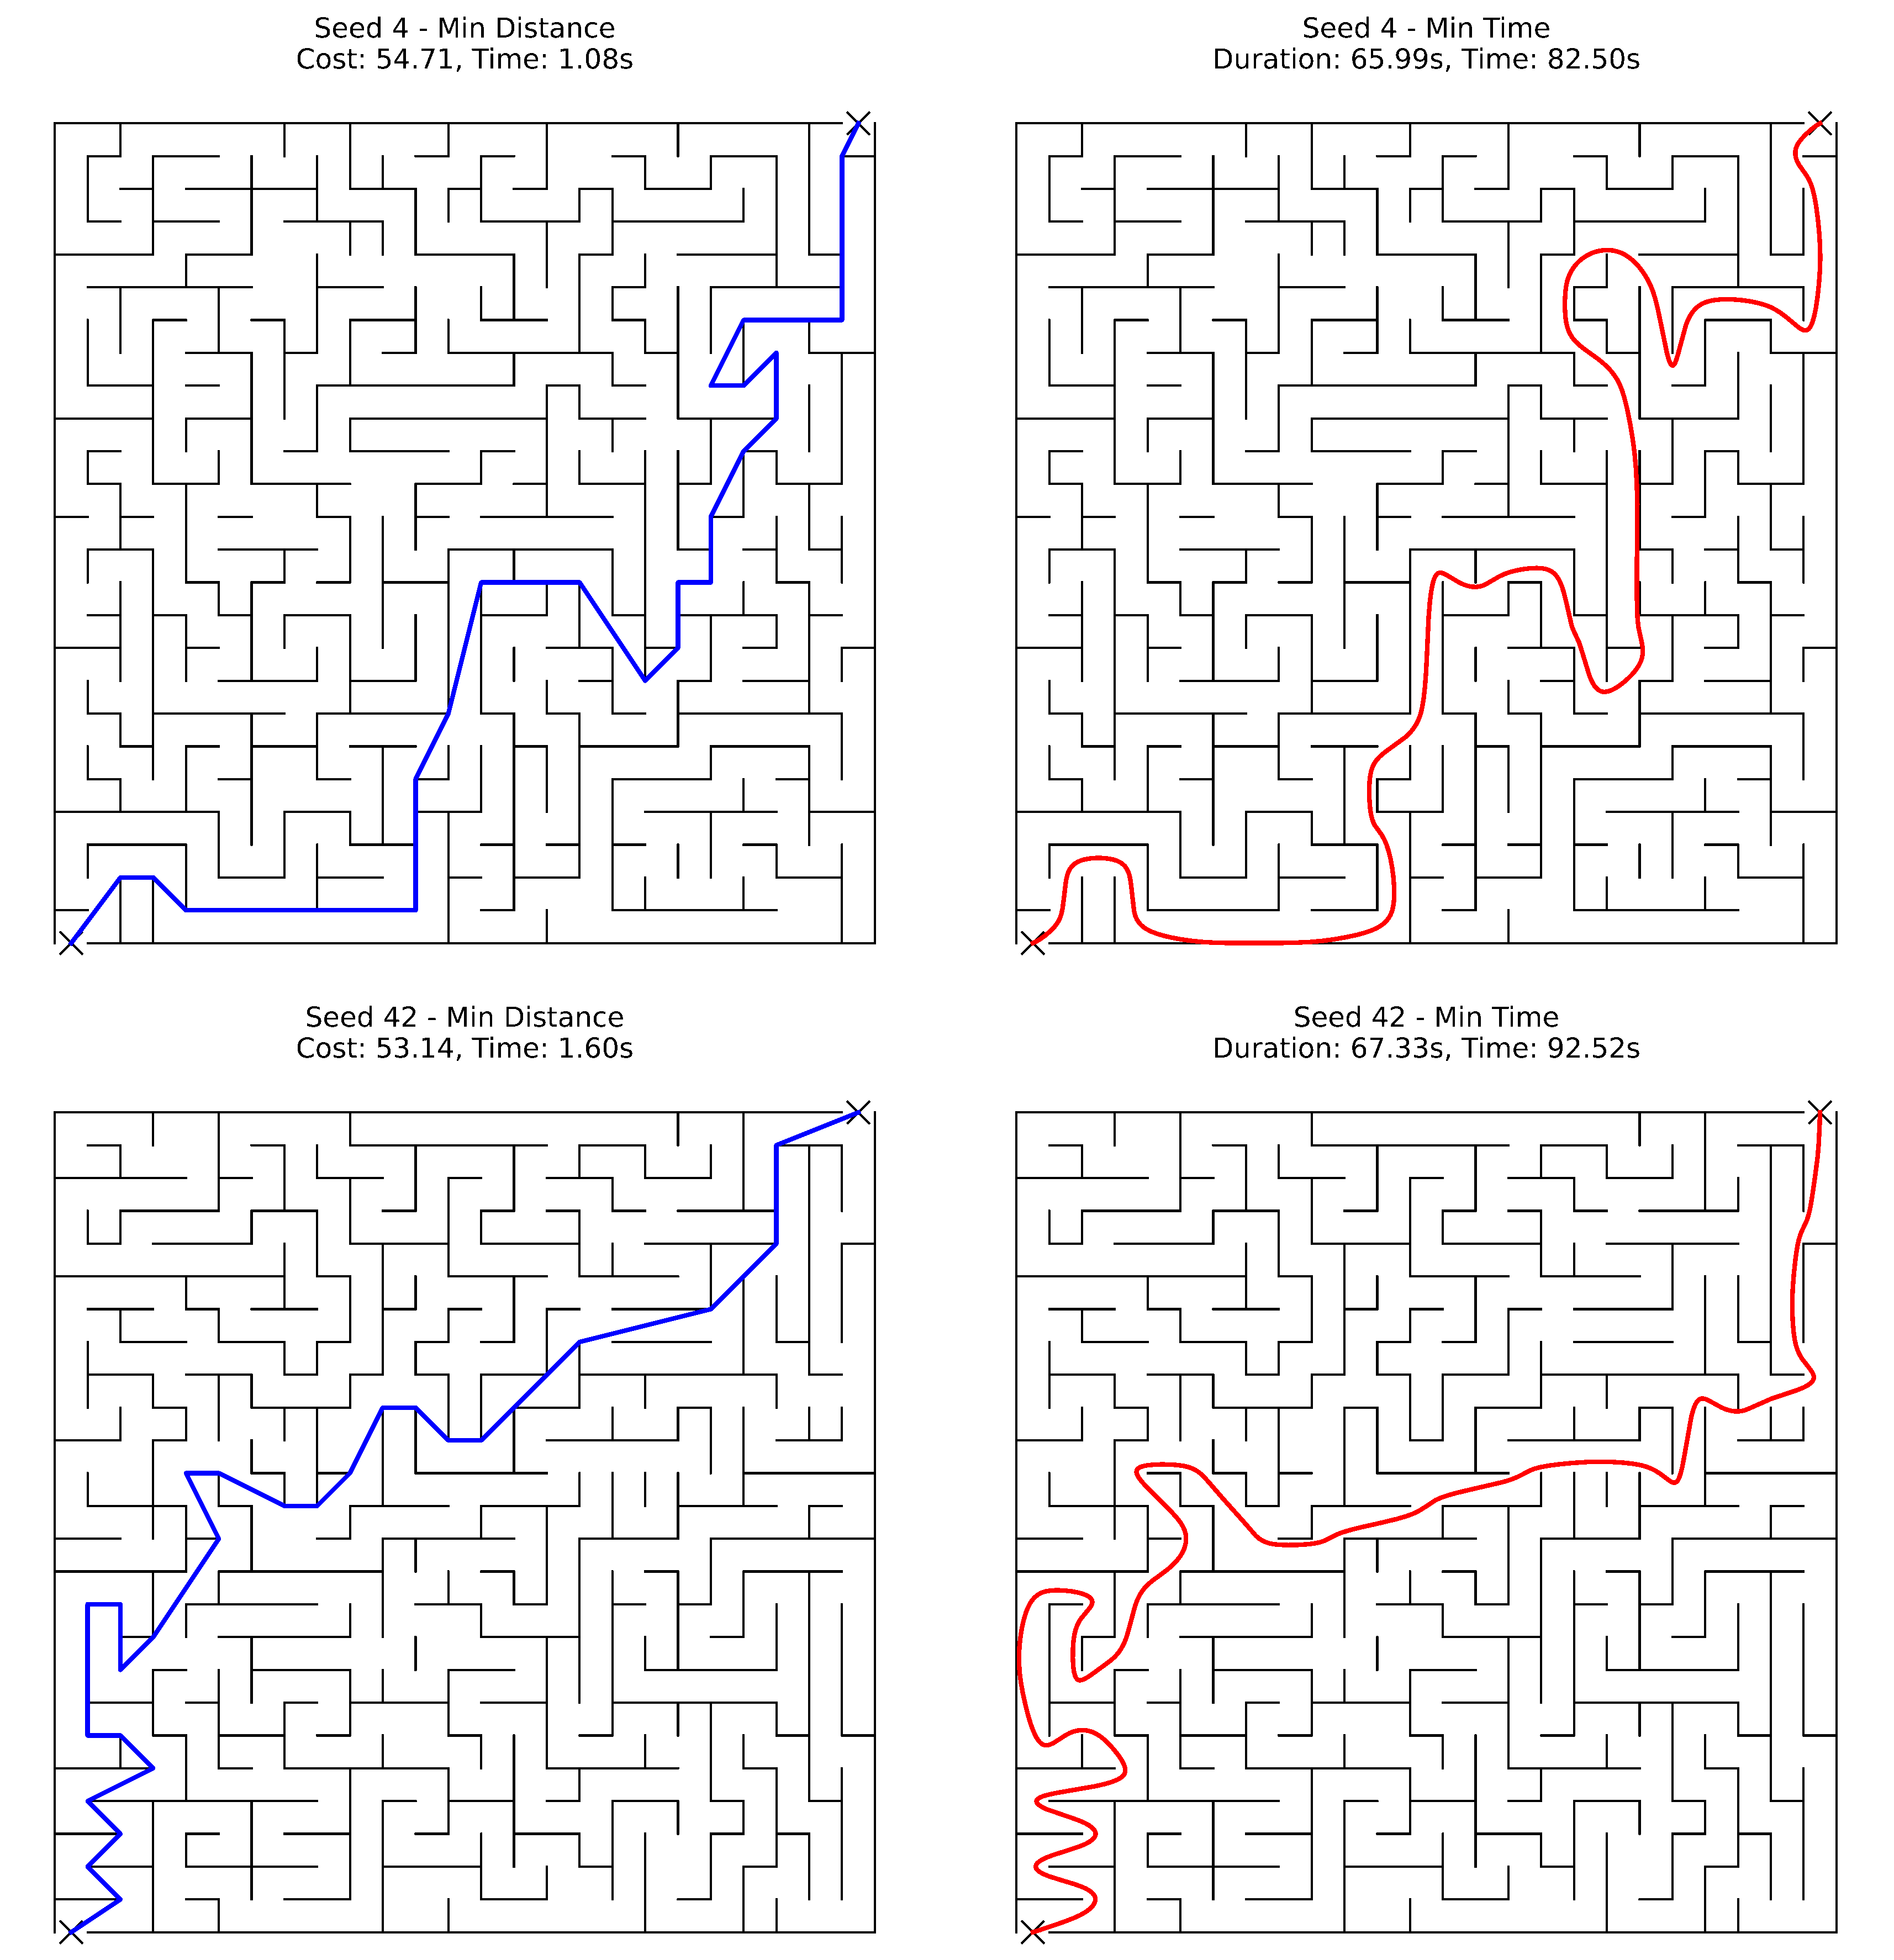
\includegraphics[width=0.8\textwidth]{./imgs/maze-1.png}\\
            {\footnotesize Khác homotopy: Bézier chọn đường \textit{dài hơn} nhưng ít cua gắt}
        \end{column}
    \end{columns}
\end{frame}

% =====================================================================
% TN1 - Slide 1: Convergence on 2D environment
% =====================================================================
\begin{frame}{TN1 — GCS-DMS: hội tụ trên môi trường 2D}
    \begin{columns}[T,onlytextwidth]
        \begin{column}{0.45\textwidth}
            \centering
            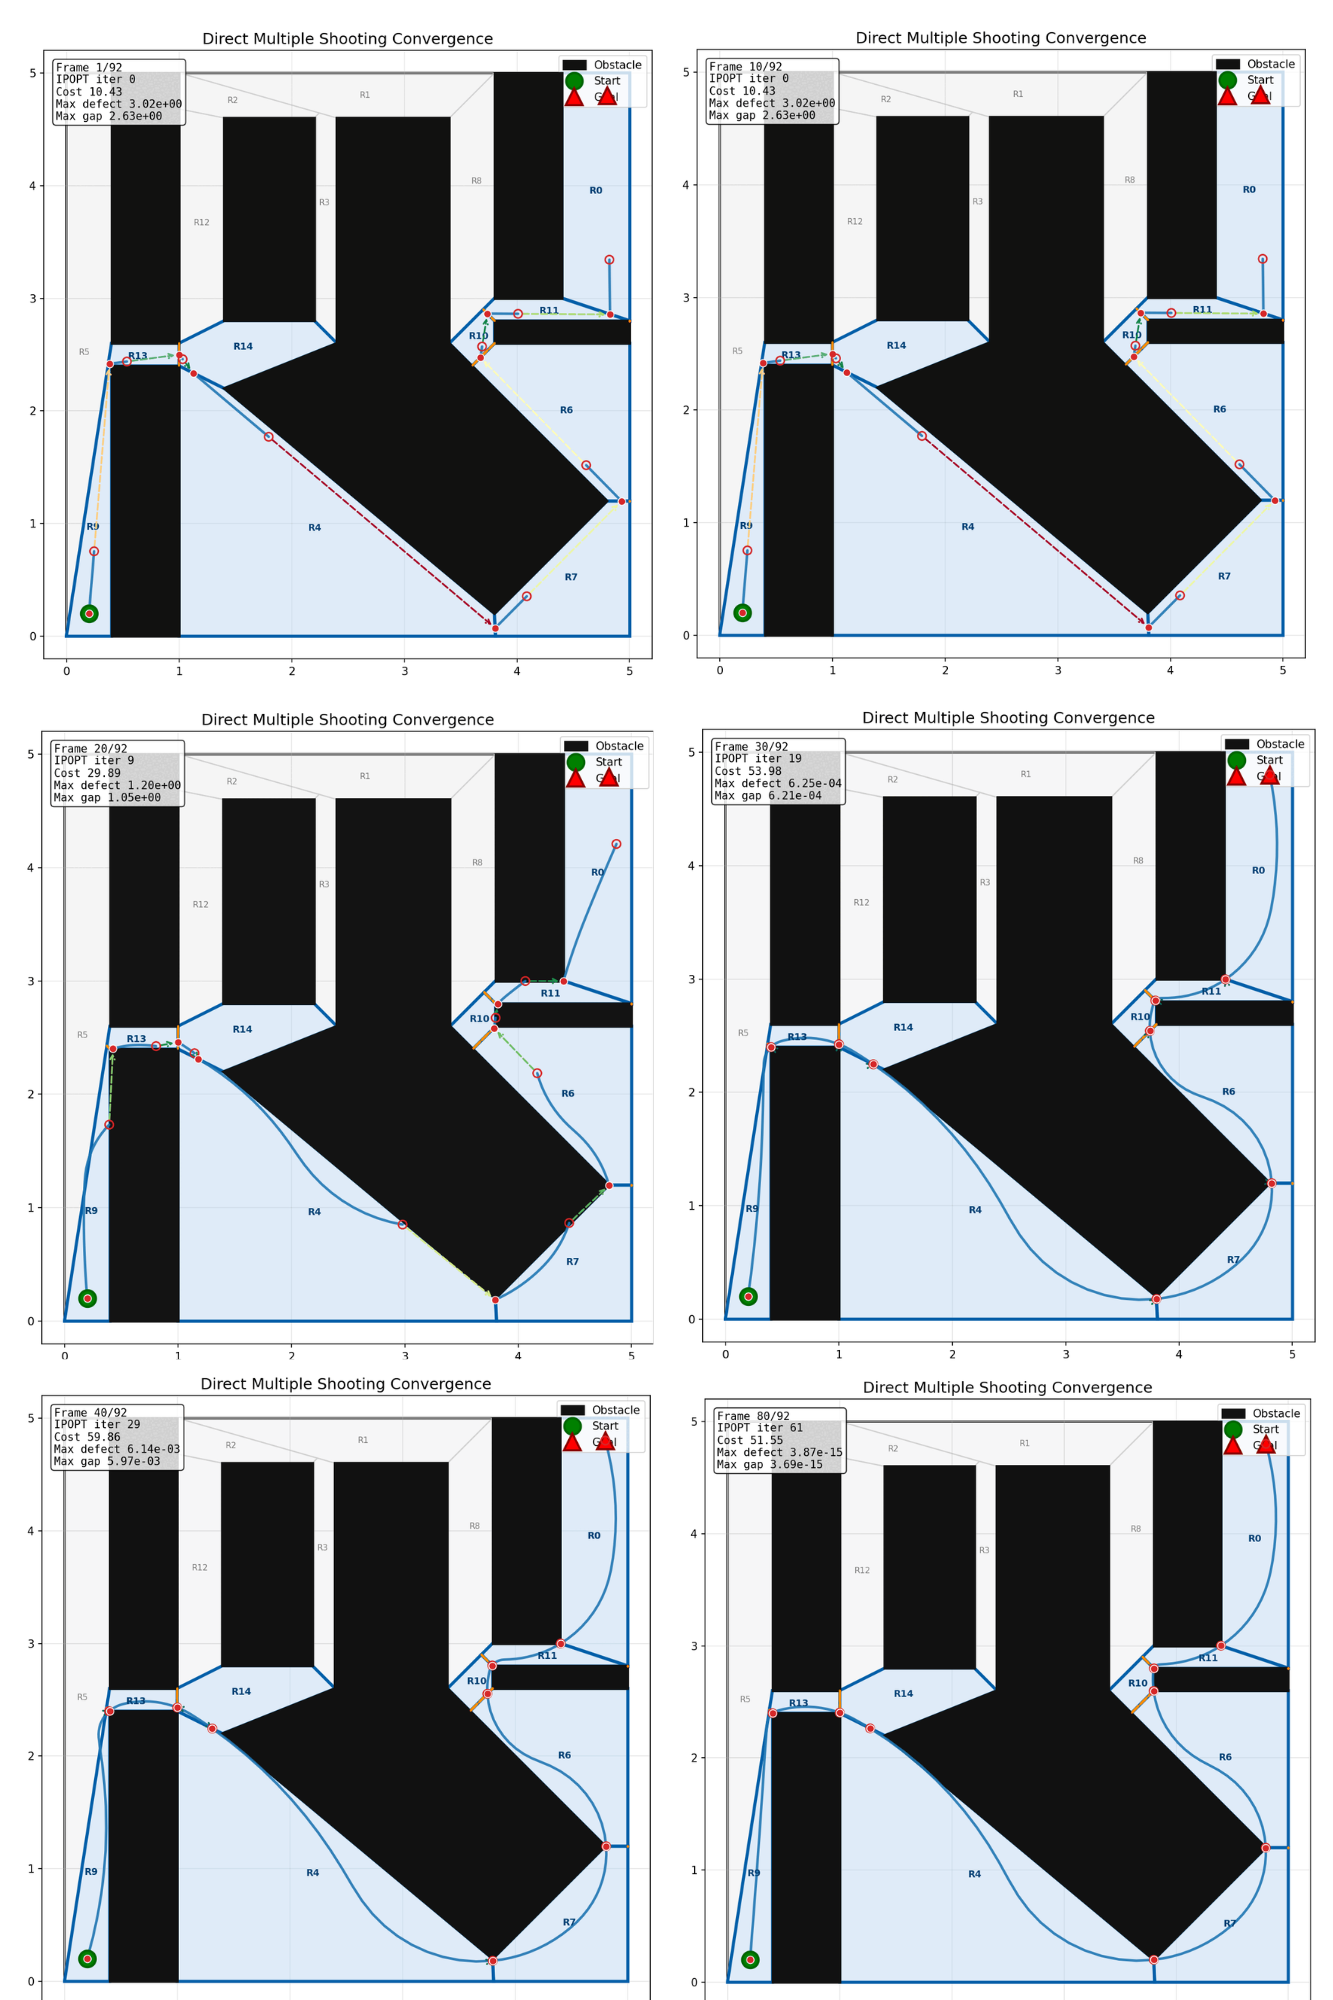
\includegraphics[height=6cm]{./imgs/dms/conv_2d.png}\\
            {\footnotesize Các khung hình: defect dynamics \& connection gap giảm dần qua các vòng IPOPT.}
        \end{column}
        \begin{column}{0.55\textwidth}
            \footnotesize
            \begin{table}
                \centering\footnotesize
                \begin{tabular}{lc}
                    \toprule
                    \textbf{Chỉ số (môi trường 2D)} & \textbf{Giá trị}                \\
                    \midrule
                    Số vùng kích hoạt               & 9                               \\
                    Thời gian thực thi $T$ (s)      & 25.47                           \\
                    Thời gian giải (s)              & 17.94                           \\
                    Cost                            & 51.55                           \\
                    \midrule
                    Defect dynamics                 & $2.47\!\times\!10^{-11}$        \\
                    Connection gap                  & $1.05\!\times\!10^{-10}$        \\
                    Vi phạm an toàn                 & $7.13\!\times\!10^{-8}$         \\
                    \bottomrule
                \end{tabular}
            \end{table}
            \begin{exampleblock}{Quan sát}
                \scriptsize Nghiệm cuối hội tụ về quỹ đạo liên tục, thỏa mãn đồng thời \textbf{động lực phi tuyến + ràng buộc an toàn} ở mức \textbf{chính xác số học} ($10^{-8}\!-\!10^{-11}$).
            \end{exampleblock}
        \end{column}
    \end{columns}
\end{frame}

% =====================================================================
% TN1 - Slide 2: Maze 15x15 with 4 seeds
% =====================================================================
\begin{frame}{TN1 — GCS-DMS: mê cung $15\!\times\!15$ (4 mẫu đại diện)}
    \begin{columns}[T,onlytextwidth]
        \begin{column}{0.6\textwidth}
            \centering
            \begin{minipage}{0.47\linewidth}
                \centering
                
\includegraphics[height=2.8cm]{./imgs/dms/maze_case_size15_kd15_seed4_animation_last_frame.png}\\
                {\scriptsize Seed 4 — log-barrier, 24 vùng}
            \end{minipage}\hfill
            \begin{minipage}{0.47\linewidth}
                \centering
                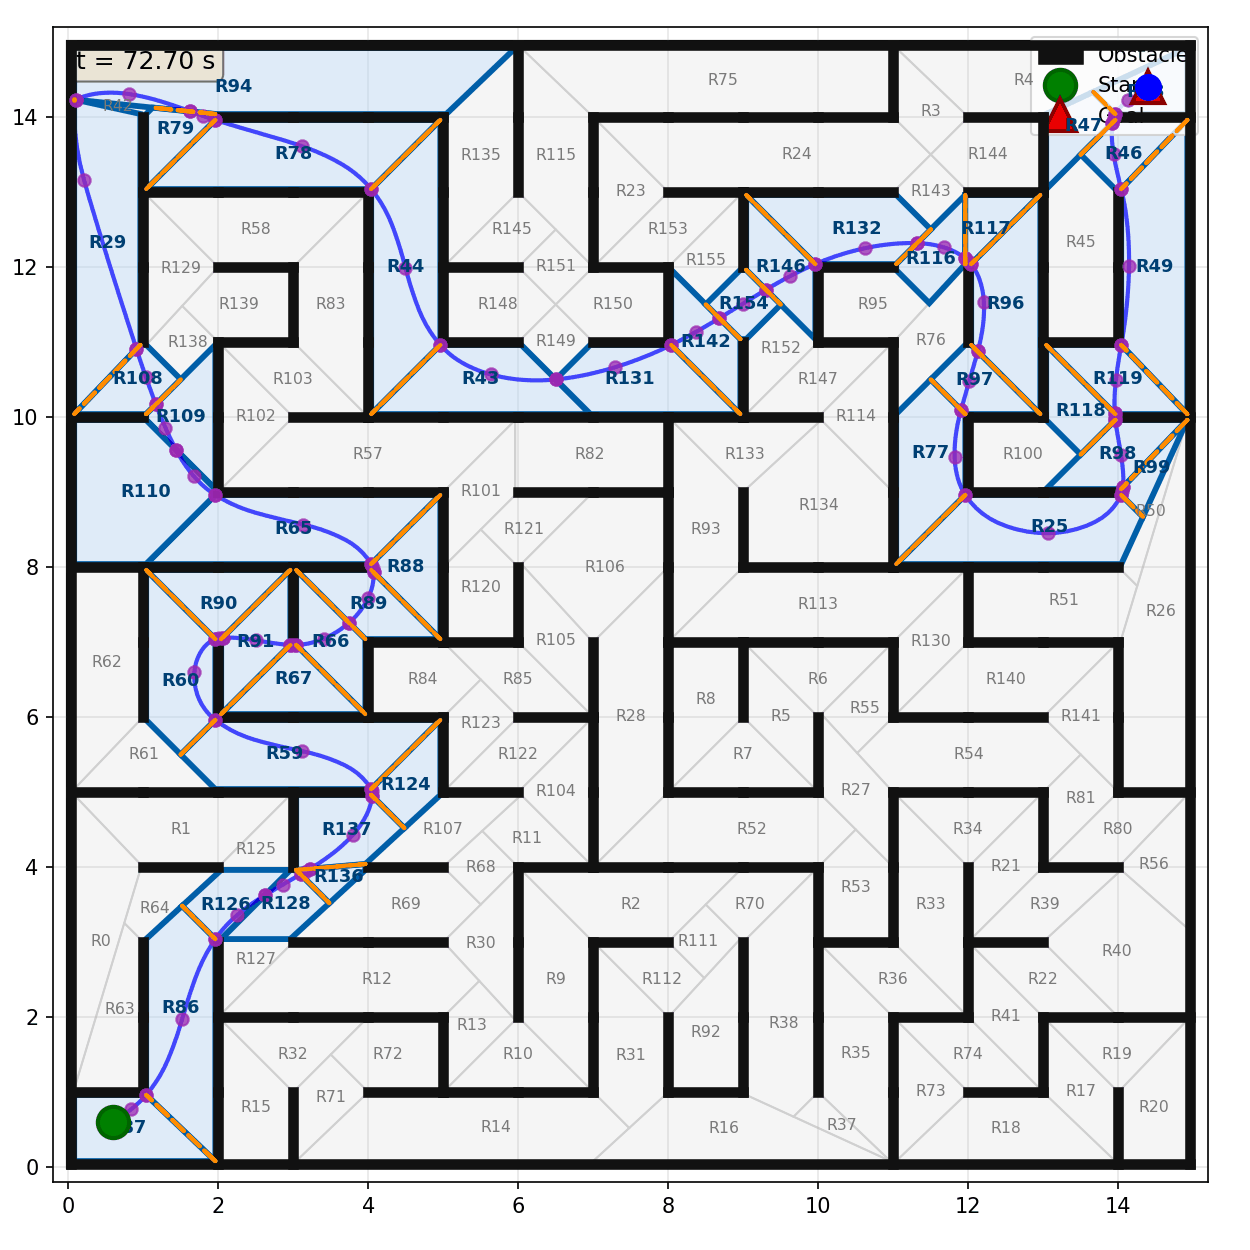
\includegraphics[height=2.8cm]{./imgs/dms/maze_case_size15_kd15_seed20_animation_last_frame.png}\\
                {\scriptsize Seed 20 — log-barrier, 44 vùng}
            \end{minipage}
            
            \begin{minipage}{0.47\linewidth}
                \centering
                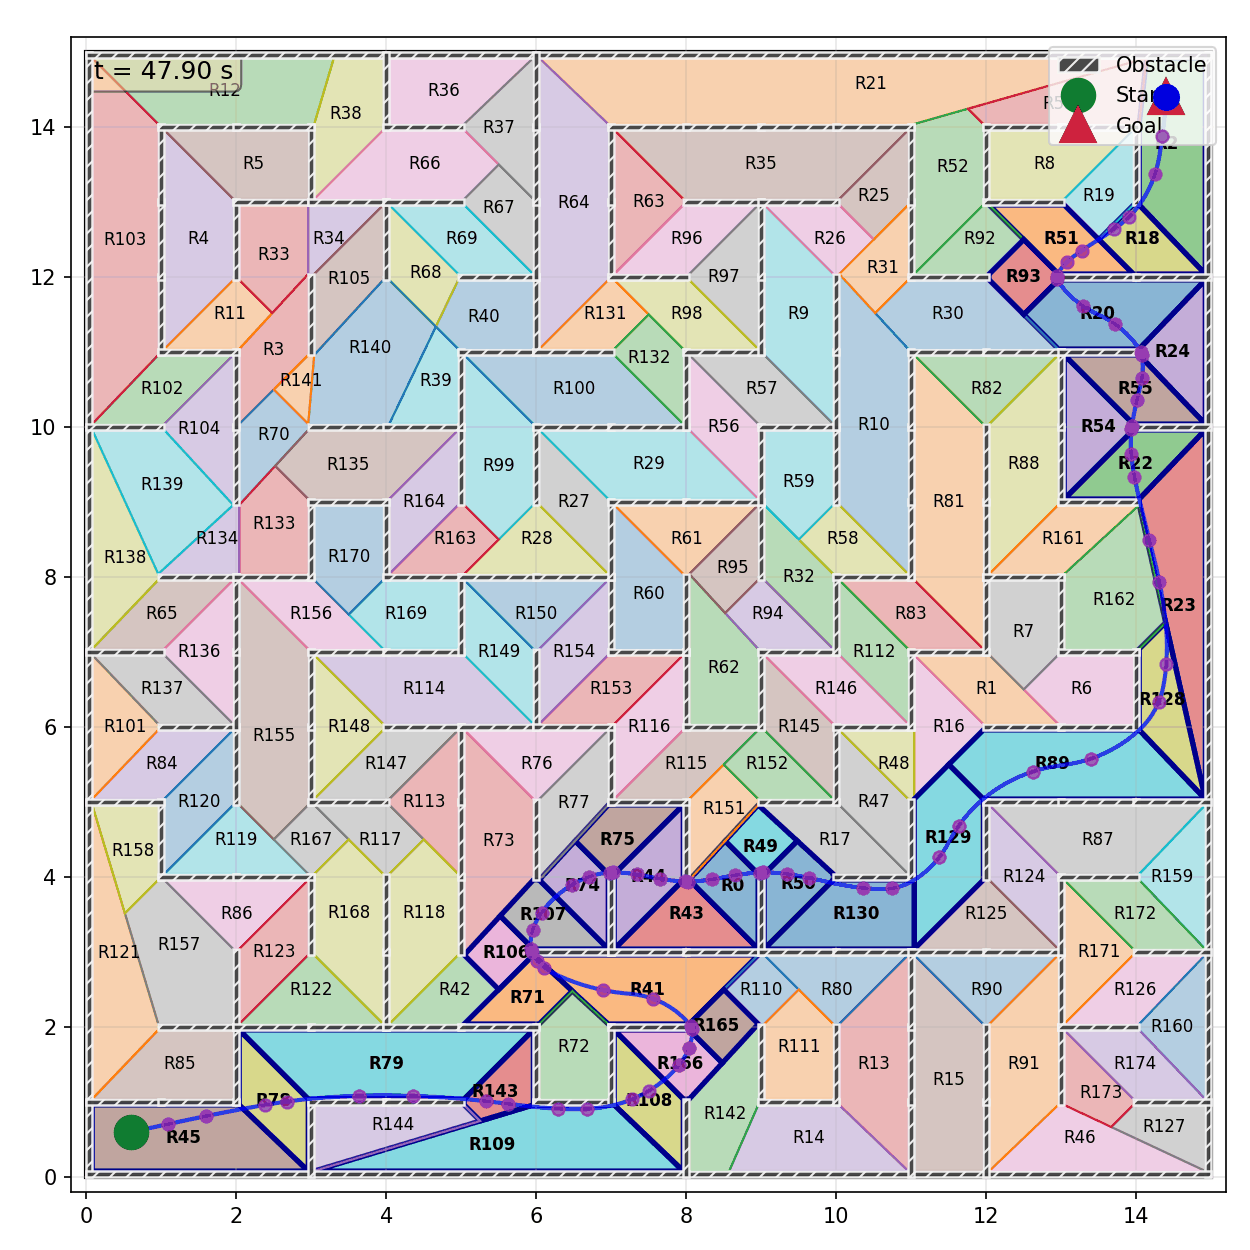
\includegraphics[height=2.8cm]{./imgs/dms/maze_case_size15_kd15_seed18_animation_last_frame.png}\\
                {\scriptsize Seed 18 — lưới điểm, 33 vùng}
            \end{minipage}\hfill
            \begin{minipage}{0.47\linewidth}
                \centering
                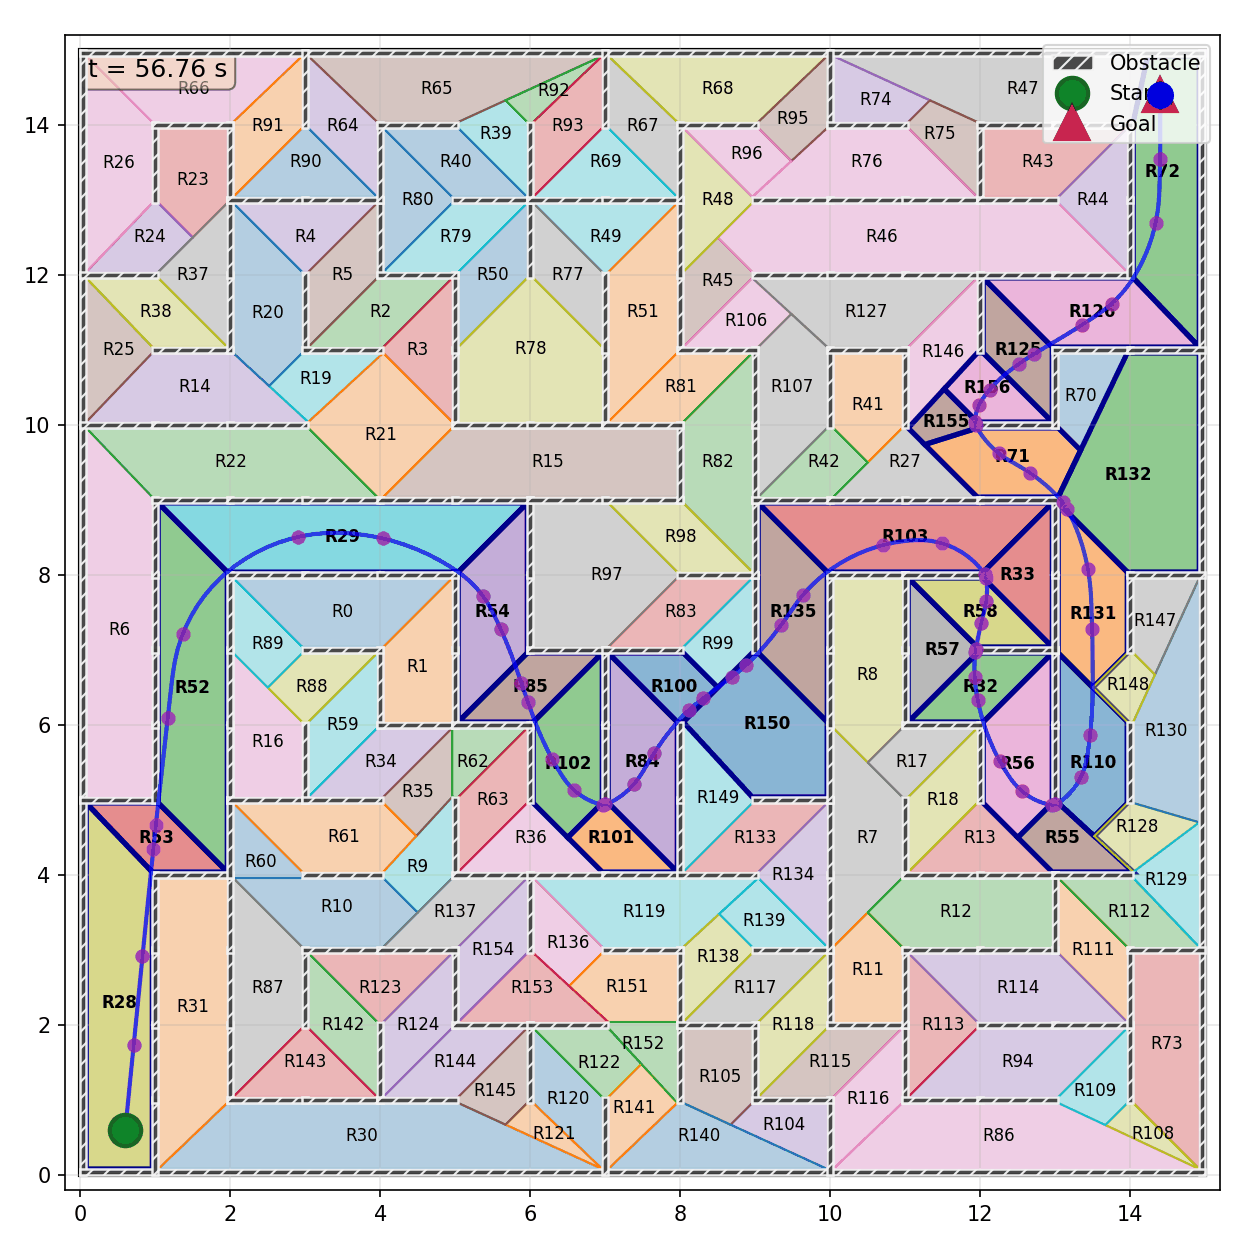
\includegraphics[height=2.8cm]{./imgs/dms/maze_case_size15_kd15_seed17_animation_last_frame.png}\\
                {\scriptsize Seed 17 — lưới điểm, 27 vùng}
            \end{minipage}\\[0.3em]
        \end{column}
        \begin{column}{0.4\textwidth}
            \begin{block}{Mô hình động lực}
                \footnotesize
                \textbf{Unicycle:} $\dot p_x = v\cos\theta,\ \dot p_y = v\sin\theta,\ \dot\theta=\omega$;\\
                $v\!\in\![-2,2],\ |\omega|\!\le\!\pi$.
            \end{block}
            \begin{exampleblock}{Tổng quát hóa}
                \footnotesize
                Tỉ lệ thành công \textbf{10/10 seed} cho cả hai cơ chế an toàn:
                \begin{itemize}\itemsep0pt
                    \item Defect $\sim 10^{-10}$
                    \item Gap $\sim 10^{-9}$
                    \item Vi phạm $\sim 10^{-8}$
                \end{itemize}
                $\Rightarrow$ \textbf{nghiệm khả thi động lực học} trên nhiều cấu trúc mê cung.
            \end{exampleblock}
        \end{column}
    \end{columns}
\end{frame}

% =====================================================================
% TN1 - Slide 3: Velocity profile insight
% =====================================================================
\begin{frame}{TN1 — Hồ sơ vận tốc \& dấu vết động lực phi tuyến}
    \begin{columns}[T,onlytextwidth]
        \begin{column}{0.6\textwidth}
            \centering
            \begin{minipage}{0.48\linewidth}
                \centering
                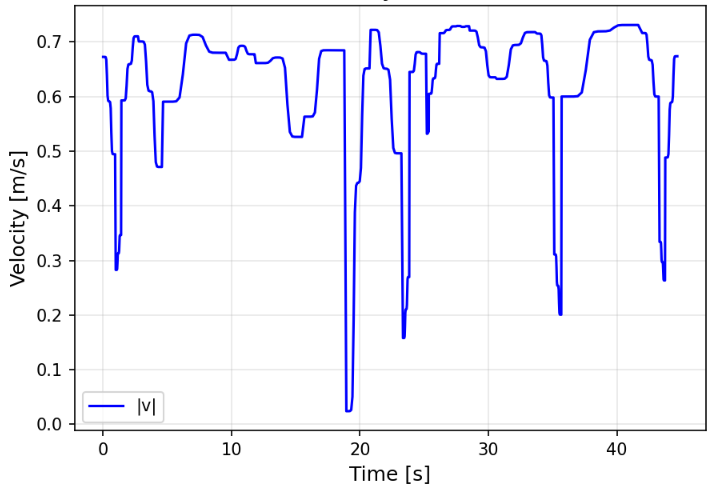
\includegraphics[width=0.9\linewidth]{./imgs/dms/seed4_vel.png}\\
                {\scriptsize $|v(t)|$ — Seed 4}
            \end{minipage}\hfill
            \begin{minipage}{0.48\linewidth}
                \centering
                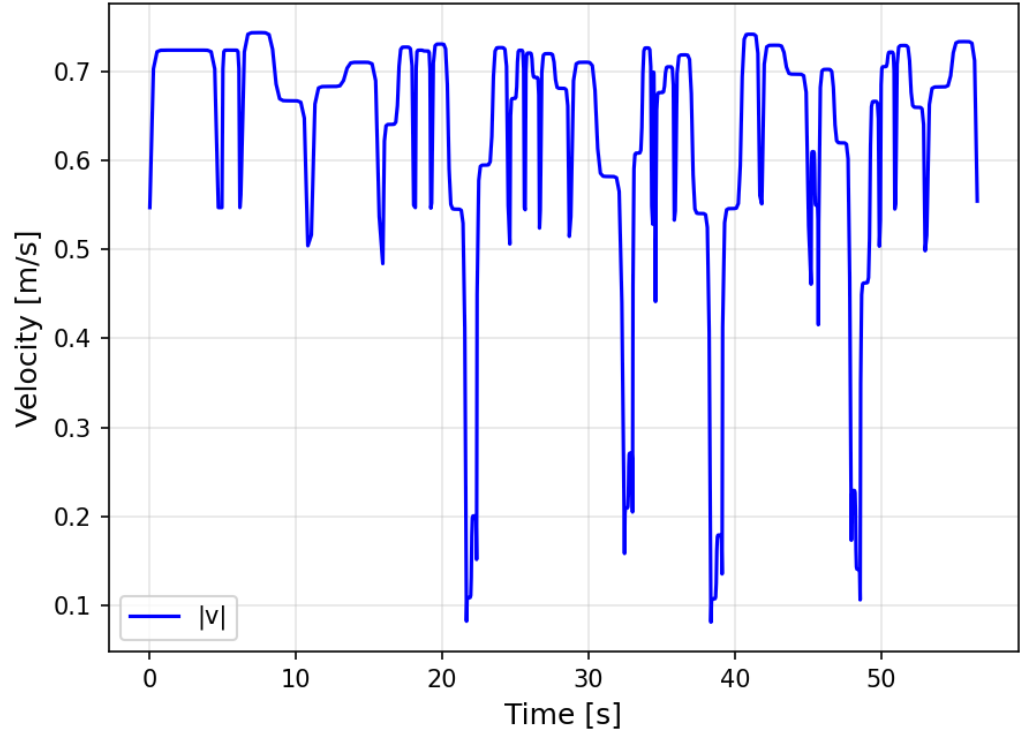
\includegraphics[width=0.9\linewidth]{./imgs/dms/seed17_vel.png}\\
                {\scriptsize $|v(t)|$ — Seed 17}
            \end{minipage}\\[0.3em]
            {\footnotesize Hồ sơ vận tốc dao động $0.6$-$0.75$ m/s, giảm sâu tại nút giao/hành lang hẹp.}
        \end{column}
        \begin{column}{0.35\textwidth}
            \begin{exampleblock}{Đặc trưng động lực Unicycle}
                \footnotesize
                Xe \textbf{tự động giảm tốc} tại:
                \begin{itemize}\itemsep0pt
                    \item Nút giao (cần đổi hướng)
                    \item Hành lang hẹp
                    \item Đoạn chuyển nhiều vùng
                \end{itemize}
                Lý do: giới hạn $|\omega|\!\le\!\omega_{\max}$ buộc giảm $v$ để có bán kính cua $\ge v/\omega_{\max}$.
            \end{exampleblock}
            \begin{alertblock}{Điểm GCS-Bézier không có}
                \scriptsize Tối ưu hình học thuần \textit{không} phản ánh được hành vi này.
            \end{alertblock}
        \end{column}
    \end{columns}
\end{frame}

% =====================================================================
% TN1 - Slide 4: Log-barrier vs finite-grid comparison
% =====================================================================
\begin{frame}{TN1 — Hai cơ chế an toàn: log-barrier vs lưới điểm}
    \footnotesize
    \begin{table}
        \centering\footnotesize
        \caption{So sánh trên cùng 10 seed mê cung $15\!\times\!15$ (giữ nguyên mọi tham số khác).}
        \begin{tabular}{lcccc}
            \toprule
            \textbf{Chế độ}     & \textbf{Tỉ lệ thành công} & \textbf{Solve TB (s)} & \textbf{Cost TB} & \textbf{Int. gap TB} \\
            \midrule
            Log-barrier         & 10/10                     & 245.51                & 118.63           & $1.4\!\times\!10^{-1}$ \\
            Lưới hữu hạn điểm   & 10/10                     & \textbf{81.60}        & \textbf{115.55}  & \textbf{$6.4\!\times\!10^{-2}$} \\
            \bottomrule
        \end{tabular}
    \end{table}

    \begin{columns}[T,onlytextwidth]
        \begin{column}{0.5\textwidth}
            \begin{block}{Log-barrier $\;-\mu\sum\log(-a_i^\top x + b_i)$}
                \footnotesize
                \begin{itemize}\itemsep0pt
                    \item[$+$] Quỹ đạo nằm \textbf{sâu} trong vùng an toàn.
                    \item[$+$] Mô hình hóa rõ về mặt lý thuyết.
                    \item[$-$] Chậm $\sim$3$\times$ do hàm log phi tuyến.
                \end{itemize}
            \end{block}
        \end{column}
        \begin{column}{0.5\textwidth}
            \begin{exampleblock}{Lưới hữu hạn điểm}
                \footnotesize
                \begin{itemize}\itemsep0pt
                    \item[$+$] Transcription trực tiếp, dễ kiểm soát.
                    \item[$+$] Nhanh \& integrality gap nhỏ hơn.
                    \item[$-$] Đảm bảo phụ thuộc số/vị trí điểm.
                \end{itemize}
            \end{exampleblock}
        \end{column}
    \end{columns}

    \vspace{0.2em}
    {\footnotesize\alert{Hai cơ chế phục vụ \textbf{hai ưu tiên khác nhau}: mô hình hóa lý thuyết vs tốc độ giải.}}
\end{frame}

% =====================================================================
% Summary slide
% =====================================================================
\begin{frame}{Tổng hợp đánh giá ba thực nghiệm}
    \begin{columns}[T,onlytextwidth]
        \begin{column}{0.33\textwidth}
            \begin{block}{TN3 — Phân hoạch}
                \footnotesize
                \begin{itemize}\itemsep0pt
                    \item ACD: \textbf{cân bằng nhất} cho 2D.
                    \item VCC: dày đặc $\Rightarrow$ giải chậm trong 2D, hữu ích cho không gian cao chiều.
                    \item Chất lượng phân hoạch \textit{quyết định trực tiếp} chi phí giải.
                \end{itemize}
            \end{block}
        \end{column}
        \begin{column}{0.33\textwidth}
            \begin{exampleblock}{TN2 — Mở rộng tổ hợp}
                \footnotesize
                \begin{itemize}\itemsep0pt
                    \item GCS-Bézier xử lý 625 ô \textbf{ổn định}.
                    \item Relaxation \textbf{chặt} $\Rightarrow$ optimality gap $=0\%$.
                    \item Bézier giúp quỹ đạo $C^2$ với chi phí $\uparrow$ $\sim$22\% so với Linear.
                \end{itemize}
            \end{exampleblock}
        \end{column}
        \begin{column}{0.33\textwidth}
            \begin{alertblock}{TN1 — Động lực phi tuyến}
                \footnotesize
                \begin{itemize}\itemsep0pt
                    \item GCS-DMS \textbf{khả thi} cho Unicycle.
                    \item Defect $\sim 10^{-10}$ — chính xác số học.
                    \item Đánh đổi: NLP phi lồi, \textit{không} bảo đảm toàn cục.
                \end{itemize}
            \end{alertblock}
        \end{column}
    \end{columns}

    \vspace{0.3em}
    \begin{block}{Vai trò bổ trợ giữa hai hướng tiếp cận}
        \footnotesize
        GCS-Bézier và GCS-DMS giải hai bài toán khác nhau (hình học lồi vs điều khiển phi tuyến). Chúng \textbf{bổ trợ} nhau: Bézier cho \textit{mở rộng tổ hợp + tối ưu toàn cục} về hình học; DMS cho \textit{tính khả thi động lực học} trên rô-bốt thực.
    \end{block}
\end{frame}

\begin{frame}{Giới hạn của GCS}
    \textbf{1. Phụ thuộc vào chất lượng phân hoạch lồi (Convex Decomposition):}
    \begin{itemize}
        \item Số lượng vùng lồi ảnh hưởng trực tiếp đến kích thước bài toán
        \item Chất lượng phân hoạch quyết định khả năng tìm được quỹ đạo tối ưu
        \item Có thể bỏ sót vùng tự do nhỏ
    \end{itemize}

    \textbf{2. Kích thước bài toán:}
    \begin{itemize}
        \item Số miền lồi lớn $\Rightarrow$ nhiều biến, chi phí tính cao
    \end{itemize}

    \textbf{3. Thách thức với môi trường động (Dynamic Environments):}
    \begin{itemize}
        \item Môi trường động: cần tái tính
        \item Thời gian tính toán hiện tại chưa phù hợp cho ứng dụng thời gian thực
    \end{itemize}
\end{frame}

% \begin{frame}{So sánh với phương pháp tối ưu khác}
%     \textbf{Tối ưu cục bộ:}
%     \begin{itemize}
%         \item CHOMP \cite{ratliff2009}: tối ưu gradient, không thoát cực trị địa phương
%         \item TrajOpt \cite{schulman2014}: Sequential Convex Programming
%     \end{itemize}

%     \textbf{GCS:}
%     \begin{itemize}
%         \item Tối ưu toàn cục nhờ relax lồi chặt
%         \item Kết hợp quyết định rời rạc và liên tục
%         \item Linh hoạt với nhiều loại ràng buộc lồi \cite{marcucci2023motion}
%     \end{itemize}

%     \vspace{0.5em}

%     \textbf{Mở rộng:}
%     \begin{itemize}
%         \item Space-Time GCS cho đa robot
%         \item Task and Motion Planning tích hợp
%         \item GCS trên đa tạp (manifold) \cite{tedrake2023}
%     \end{itemize}
% \end{frame}

\section{Tổng kết}

\begin{frame}{Tổng kết và Hướng nghiên cứu tương lai}
    \begin{columns}[T, onlytextwidth]
        % Cột trái: Kết luận
        \begin{column}{0.48\textwidth}
            \textbf{1. Tổng kết}
            \vspace{0.2cm}
            \begin{itemize}
                \item \textbf{Mô hình hóa:} Hoạch định chuyển động trong môi trường có vật cản bằng tối ưu lồi.
                \item Hiểu rõ và tái thực hiện \textbf{cấu trúc GCS} vào bài toán hoạch định chuyển
                      động trong không gian 2D.
                \item \textbf{Đối chiếu:} Các giải thuật phân hoạch và kiểm chứng độ tối ưu.
            \end{itemize}
        \end{column}

        % Cột phải: Hướng phát triển
        \begin{column}{0.48\textwidth}
            \textbf{2. Lộ trình phát triển}
            \vspace{0.2cm}
            \begin{itemize}
                \item Hoàn thiện mô hình hoàn chỉnh cho hoạch định chuyển động cho không gian cao
                      chiều bằng GCS.
                \item Tích hợp trên robot thực tế.
                \item \textbf{Refinement:} Vận dụng \textbf{Multiple Shooting} hậu xử lý.
                \item \textbf{Benchmarking:} Đánh giá đối chứng quy mô lớn với RRT* và PRM.
            \end{itemize}
        \end{column}
    \end{columns}

\end{frame}

\begin{frame}[allowframebreaks]{Tài liệu tham khảo}
    \begin{thebibliography}{99}

        \bibitem{marcucci2023motion}
        Tobia Marcucci et al., ``Motion planning around obstacles with convex optimization,'' \emph{Science Robotics}, vol. 8, no. 84, 2023. (arXiv:2205.04422)

        \bibitem{marcucci2024shortest}
        Tobia Marcucci et al., ``Shortest Paths in Graphs of Convex Sets,'' \emph{SIAM Journal on Optimization}, vol. 34, no. 1, 2024. (arXiv:2101.11565)

        \bibitem{tedrake2023}
        Russ Tedrake, \emph{Underactuated Robotics -- Chapter 6: Motion Planning}, MIT Course Notes, 2023. \url{http://manipulation.csail.mit.edu/trajectories.html}

        \bibitem{deits2015}
        Robin Deits and Russ Tedrake, ``Computing Large Convex Regions of Obstacle-Free Space through Semidefinite Programming,'' \emph{Algorithmic Foundations of Robotics XI}, 2015.

        % Approximating Robot Configuration Spaces with few Convex Sets using Clique Covers of Visibility Graphs
        % Peter Werner, Alexandre Amice, Tobia Marcucci, Daniela Rus, Russ Tedrake
        \bibitem{vcc2023}
        Peter Werner et al., ``Approximating Robot Configuration Spaces with Few Convex Sets using Clique Covers of Visibility Graphs,'' \emph{Robotics: Science and Systems (RSS)}, 2023. (arXiv:2302.05402)

        \bibitem{farin2002}
        Gerald Farin, \emph{Curves and Surfaces for CAGD: A Practical Guide}, 5th ed., Morgan Kaufmann, 2002.

        \bibitem{kavraki1996}
        Lydia E. Kavraki et al., ``Probabilistic roadmaps for path planning in high-dimensional configuration spaces,'' \emph{IEEE Transactions on Robotics and Automation}, vol. 12, no. 4, 1996.

        \bibitem{lavalle1998}
        Steven M. LaValle, ``Rapidly-exploring random trees: A new tool for path planning,'' Technical Report, Iowa State University, 1998.

        \bibitem{lien1994approximate}
        Lydia E. Lien and N. M. Amato, ``Approximate convex decomposition of polygons,'' \emph{Computational Geometry}, vol. 29, no. 4, 2004.

        \bibitem{schulman2014}
        John Schulman et al., ``Motion planning with sequential convex optimization and convex collision checking,'' \emph{The International Journal of Robotics Research}, vol. 33, no. 9, 2014.

        \bibitem{ratliff2009}
        Nathan Ratliff et al., ``CHOMP: Gradient optimization techniques for efficient motion planning,'' \emph{IEEE International Conference on Robotics and Automation (ICRA)}, 2009.

        \bibitem{motionplanning2022}
        Steven M. LaValle, \emph{Planning Algorithms}, Cambridge University Press, 2006.

        % Lectures on Robotic Planning and Kinematics
        % Francesco Bullo and Stephen L. Smith
        \bibitem{ecd_lectures}
        Francesco Bullo and Stephen L. Smith, \emph{Lectures on Robotic Planning and Kinematics}, 2022. \url{https://motion.me.ucsb.edu/lectures/}

        %         A simple and fast incremental
        % randomized algorithm for
        % computing trapezoidal
        % decompositions and for
        % triangulating polygons
        % Raimund Seidel** **

        \bibitem{seidel_decompose}
        Raimund Seidel, ``A simple and fast incremental randomized algorithm for computing trapezoidal decompositions and for triangulating polygons,'' \emph{Computational Geometry}, vol. 1, no. 1, 1991.
    \end{thebibliography}
\end{frame}

\begin{frame}[plain]
    \begin{center}
        {\Huge Cảm ơn!}

        \vspace{2em}

        {\large Câu hỏi và thảo luận}
    \end{center}
\end{frame}

\begin{frame}{Appendix}
    \begin{center}
        \Huge Phụ lục
    \end{center}
\end{frame}

\begin{frame}{Độ trơn (smoothness) của Quỹ đạo}
    \begin{itemize}
        \item \textbf{Định nghĩa:} Là mức độ biến thiên liên tục của quỹ đạo $q(t)$ theo thời gian.
        \item \textbf{Tính liên tục $C^k$:}
              \begin{itemize}
                  \item $C^0$: Liên tục về vị trí (không nhảy vọt).
                  \item $C^1$: Liên tục về vận tốc (không đổi hướng đột ngột).
                  \item $C^2$: Liên tục về gia tốc (không thay đổi lực đột ngột).
                  \item $C^3$: Liên tục về Jerk (độ giật).
              \end{itemize}
    \end{itemize}
    \begin{figure}
        \centering
        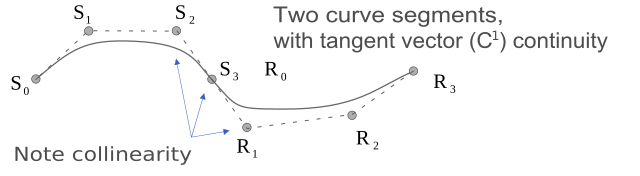
\includegraphics[width=0.6\linewidth]{./imgs/smoothness.png}
        \caption{Minh họa các mức độ độ trơn $C^0$, $C^1$}
    \end{figure}
\end{frame}

\begin{frame}{GCS vs. MICP truyền thống}
    \small
    \textbf{1. MICP Truyền thống}
    \begin{itemize}
        \item \textbf{Cơ chế:} Chia quỹ đạo thành các đoạn cố định. Với mỗi đoạn, phải gán nó vào 1 trong $|I|$ vùng an toàn thông qua biến nhị phân.
        \item \textbf{Hệ quả:} Để đảm bảo tính tổng quát (quỹ đạo có thể đi qua mọi vùng), số biến nhị phân cần là $|I| \times |I| = |I|^2$.
        \item \textbf{Thực tế:} Với 625 ô, cần \textbf{390625 biến} $\rightarrow$ Không thể giải.
    \end{itemize}

    \hrulefill

    \textbf{2. GCS: Tiếp cận dựa trên luồng đồ thị (Flow-based)}
    \begin{itemize}
        \item \textbf{Cơ chế:} Chỉ tạo biến nhị phân cho các \textbf{cạnh (edges)} nối giữa các vùng tiếp giáp nhau. Quỹ đạo được xem như một luồng chạy từ nguồn đến đích trên đồ thị.
        \item \textbf{Ưu điểm hình học:} Trong không gian 2D, mỗi vùng chỉ tiếp giáp với một số ít vùng lân cận (hệ số bậc đồ thị thấp).
        \item \textbf{Hệ quả:} Số biến nhị phân tỉ lệ thuận với số cạnh $|E| \approx 2|I|$.
        \item \textbf{Thực tế:} Với 625 ô, chỉ cần \textbf{1250 biến} $\rightarrow$ Giải được trong thời gian thực.
    \end{itemize}
\end{frame}

\begin{frame}{Appendix}
    \begin{center}
        \Huge Đường cong Bézier
    \end{center}
\end{frame}

\begin{frame}{1. Định nghĩa và Tính chất Hình học}
    \begin{block}{Đa thức Bernstein \& Đường cong Bézier}
        Đường cong Bézier bậc $d$ được xây dựng từ tập $d+1$ điểm điều khiển $\gamma_k \in \mathbb{R}^n$:
        \begin{equation*}
            \gamma(s) := \sum_{k=0}^d \beta_{k,d}(s)\gamma_k, \quad s \in [0, 1]
        \end{equation*}
        Trong đó, đa thức Bernstein là $\beta_{k,d}(s) := \binom{d}{k} s^k(1-s)^{d-k}$.
    \end{block}

    \begin{columns}
        \begin{column}{0.6\textwidth}
            \begin{itemize}
                \item \textbf{Giá trị điểm cuối:} $\gamma(0) = \gamma_0$ và $\gamma(1) = \gamma_d$.
                \item \textbf{Tính chất bao lồi:} $\gamma(s) \in \text{conv}(\{\gamma_k\}_{k=0}^d)$.
                \item \textbf{GCS Insight:} Ràng buộc an toàn liên tục $\gamma(s) \in X_v$ được đảm bảo nếu $\gamma_k \in X_v, \forall k$.
            \end{itemize}
        \end{column}
        \begin{column}{0.4\textwidth}
            % Chèn hình minh họa tại đây
            \centering
            \begin{tikzpicture}[scale=0.8]
                \draw[gray, dashed] (0,0) -- (1,2) -- (3,2.5) -- (4,0.5);
                \draw[blue, thick] (0,0) .. controls (1,2) and (3,2.5) .. (4,0.5);
                \filldraw[red] (0,0) circle (2pt) node[below]{$\gamma_0$};
                \filldraw[black] (1,2) circle (2pt) node[above]{$\gamma_1$};
                \filldraw[black] (3,2.5) circle (2pt) node[above]{$\gamma_2$};
                \filldraw[red] (4,0.5) circle (2pt) node[below]{$\gamma_3$};
            \end{tikzpicture}
            \captionof{figure}{\footnotesize Minh họa bao lồi}
        \end{column}
    \end{columns}
\end{frame}

% Slide 2: Đạo hàm và Tối ưu hóa trong GCS
\begin{frame}{2. Đạo hàm và Tối ưu hóa trong GCS}
    \begin{itemize}
        \item \textbf{Đạo hàm (Hodograph):}
              $\dot{\gamma}(s)$ cũng là một đường cong Bézier bậc $d-1$:
              \begin{equation*}
                  \dot{\gamma}(s) = \sum_{k=0}^{d-1} \beta_{k,d-1}(s) \dot{\gamma}_k, \quad \text{với } \dot{\gamma}_k = d(\gamma_{k+1} - \gamma_k)
              \end{equation*}
              \textit{Hệ quả:} Các giới hạn vận tốc/gia tốc trở thành các ràng buộc tuyến tính trên sai phân điểm điều khiển.

              \vspace{0.3cm}
        \item \textbf{Tích phân của hàm lồi (Cost Bound):}
              Đối với hàm chi phí lồi $f$, ta có cận trên hữu hạn:
              \begin{equation*}
                  \int_0^1 f(\gamma(s))ds \le \frac{1}{d+1} \sum_{k=0}^d f(\gamma_k)
              \end{equation*}
    \end{itemize}

    % \begin{alertblock}{Kết luận ứng dụng}
    %     Cấu trúc này cho phép đưa bài toán tối ưu hóa quỹ đạo liên tục về dạng \textbf{Quy hoạch lồi hỗn hợp số nguyên (MICP)}, giúp giải quyết hiệu quả các bài toán tránh va chạm và ràng buộc động lực học.
    % \end{alertblock}
\end{frame}

\begin{frame}{Tham số hóa quỹ đạo bằng đường Bézier}
    \begin{itemize}
        \item Mỗi đoạn quỹ đạo trong $Q_i$ là đường cong Bézier bậc $m$
        \item Xác định bởi $m+1$ điểm điều khiển $\gamma_0, \ldots, \gamma_m \in Q_i$
        \item $\gamma_0 = x_i^{\text{in}}$ và $\gamma_m = x_i^{\text{out}}$
    \end{itemize}

    \begin{block}{Tính chất bao lồi của đường Bézier}
        Đường cong Bézier luôn nằm trong bao lồi của các điểm điều khiển \cite{farin2002}. Do đó, nếu tất cả điểm điều khiển thuộc miền lồi $Q_i$, toàn bộ đường cong cũng nằm trong $Q_i$ và tránh va chạm.
    \end{block}

    \begin{itemize}
        \item Có thể áp đặt ràng buộc liên tục đạo hàm tại điểm nối để quỹ đạo trơn tru
              ($C^1, C^2, \ldots$) \cite{marcucci2023motion}
    \end{itemize}
\end{frame}

\begin{frame}{VCC - Giải quyết Vấn đề Seeding}
    \textbf{Quy trình 4 bước:}
    \begin{enumerate}
        \item Lấy mẫu $n$ điểm trong $C_{free}$
        \item Xây dựng đồ thị khả kiến (visibility graph)
        \item Tìm lớp phủ clique (MAXCLIQUE + ILP)
        \item Khởi tạo ellipsoid và lấp đầy (IRIS-like)
    \end{enumerate}

    \vspace{0.5em}
    \textbf{Ý tưởng cốt lõi:} Điểm ``nhìn thấy'' nhau $\Rightarrow$ có khả năng cùng vùng lồi

    \vspace{0.5em}
    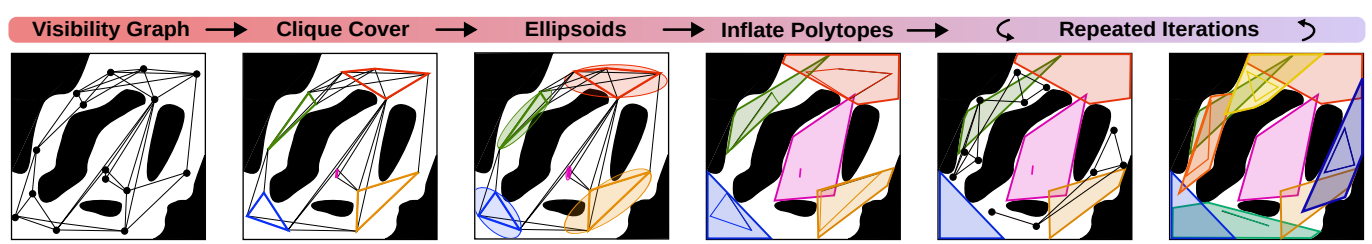
\includegraphics[width=\textwidth]{./imgs/VCC.png}

\end{frame}

\begin{frame}{VCC - Bước 1: Lấy mẫu \& Xây dựng Đồ thị Khả kiến}
    \begin{columns}[c]
        \column{0.45\textwidth}
        \centering
        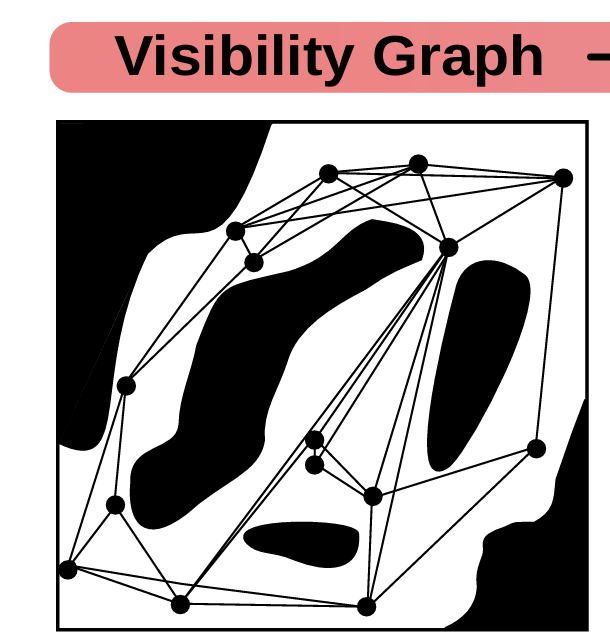
\includegraphics[width=\textwidth]{./imgs/VCC-1.png}

        \column{0.5\textwidth}
        \textbf{Visibility Graph Construction:}
        \begin{itemize}
            \item Lấy mẫu $n$ điểm ngẫu nhiên trong $C_{free}$
            \item Tạo cạnh giữa hai điểm nếu đoạn thẳng nối chúng không va chạm
            \item Xây dựng đồ thị khả kiến (visibility graph)
        \end{itemize}

        \vspace{0.5em}
        \begin{exampleblock}{Định nghĩa}
            \textbf{Visibility graph:} Đồ thị có cạnh nối hai đỉnh khi đoạn thẳng nối chúng nằm hoàn toàn trong không gian tự do
        \end{exampleblock}
    \end{columns}
\end{frame}

\begin{frame}{VCC - Bước 2: Tìm Lớp phủ Clique}
    \begin{columns}[c]
        \column{0.45\textwidth}
        \centering
        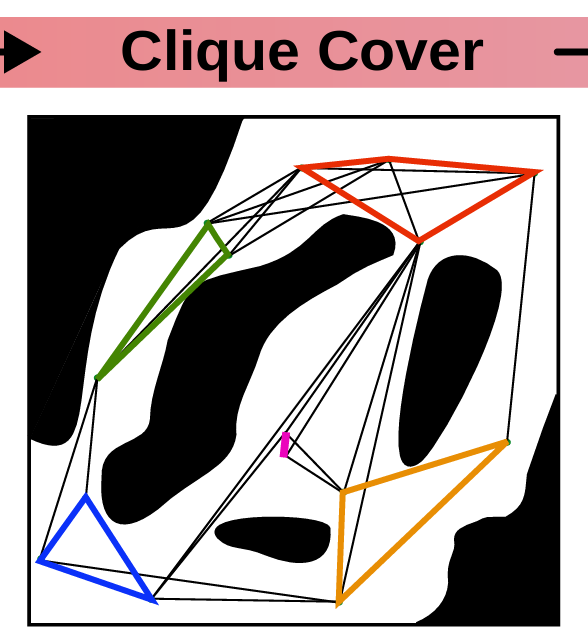
\includegraphics[width=\textwidth]{./imgs/VCC-2.png}

        \column{0.5\textwidth}

        \begin{exampleblock}{Định nghĩa Clique}
            \small
            Tập con đồ thị mà mọi cặp đỉnh đều có cạnh nối (đồ thị con đầy đủ)
        \end{exampleblock}

        \vspace{0.5em}
        \textbf{Truncated Clique Cover:}
        \begin{itemize}
            \item Tìm các clique lớn ($\geq s_{min}$ đỉnh)
            \item MAXCLIQUE algorithm (ILP)
            \item Lặp đến khi clique còn lại quá nhỏ
        \end{itemize}
    \end{columns}
\end{frame}

\begin{frame}{VCC - MAXCLIQUE Problem}

    \textbf{Mục tiêu:} Tìm clique lớn nhất trong visibility graph

    \vspace{0.5em}
    \begin{block}{Integer Linear Programming Formulation}
        \small
        \[
            \begin{aligned}
                \max \quad        & \sum_{i=1}^{K} b_i                                  \\
                \text{s.t.} \quad & b_i + b_j \leq 1, \quad \forall \{i,j\} \in \bar{E} \\
                                  & b_i \in \{0, 1\}, \quad \forall i = 1, \ldots, K
            \end{aligned}
        \]
    \end{block}

    \vspace{0.5em}
    \textbf{Giải thích:}
    \begin{itemize}
        \item $b_i = 1$ nếu đỉnh $i$ được chọn vào clique, $b_i = 0$ nếu không
        \item $\bar{E}$: tập các cặp đỉnh \textbf{không} có cạnh nối ($\{i,j\} \notin E$)
        \item Ràng buộc: Hai đỉnh chỉ được chọn cùng lúc nếu chúng có cạnh nối
    \end{itemize}

\end{frame}

\begin{frame}{VCC - Thuật toán Tham lam}

    \textbf{Quy trình lặp:}
    \begin{enumerate}
        \item Giải ILP để tìm clique lớn nhất trong đồ thị hiện tại
        \item Thêm clique vào lớp phủ $\mathcal{T}$
        \item Loại bỏ các đỉnh của clique khỏi đồ thị
        \item Lặp lại cho đến khi clique lớn nhất còn lại có kích thước $< s_{min}$
    \end{enumerate}

    \vspace{0.5em}
    \textbf{Truncated Cover:}
    \begin{itemize}
        \item Chỉ giữ lại các clique lớn ($\geq s_{min}$ đỉnh)
        \item Clique nhỏ không mang thông tin hữu ích
        \item Một số đỉnh có thể không thuộc clique nào
    \end{itemize}

    \vspace{0.5em}
    \textbf{Lý do:} Các clique nhỏ thường không đại diện cho vùng lồi có ý nghĩa

\end{frame}

\begin{frame}{VCC - Bước 3: Khởi tạo Ellipsoid}
    \begin{columns}[c]
        \column{0.45\textwidth}
        \centering
        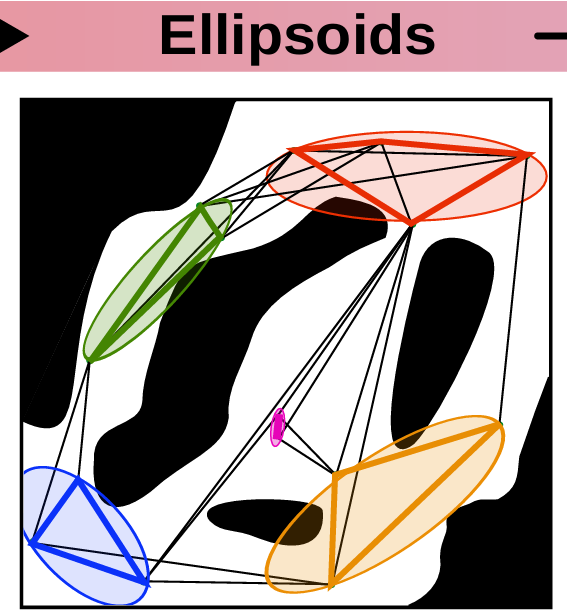
\includegraphics[width=\textwidth]{./imgs/VCC-3.png}

        \column{0.5\textwidth}
        \textbf{Ellipsoid Initialization:}
        \begin{itemize}
            \item Tính ellipsoid có thể tích nhỏ nhất bao quanh tất cả điểm trong clique
            \item Cung cấp tâm (seed point) cho bước tiếp theo
            \item Xác định hình dạng ban đầu (các trục chính)
        \end{itemize}
    \end{columns}
\end{frame}

\begin{frame}{VCC - Bước 4: Lấp đầy thành Đa diện}
    \begin{columns}[c]
        \column{0.45\textwidth}
        \centering
        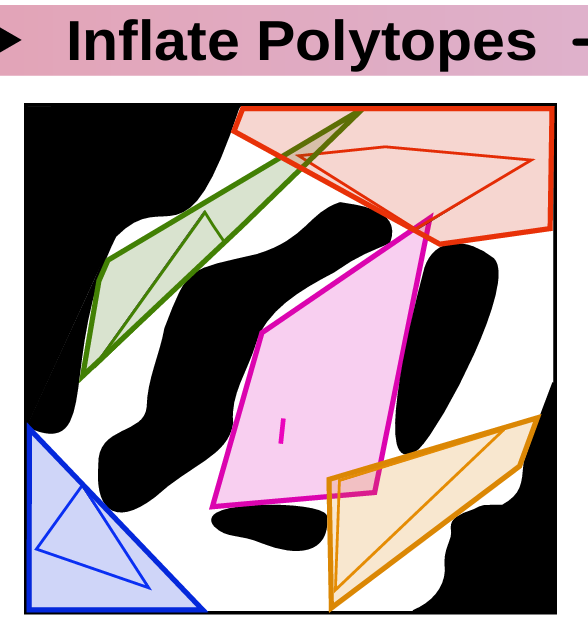
\includegraphics[width=\textwidth]{./imgs/VCC-4.png}

        \column{0.5\textwidth}
        \textbf{Inflation Process:}
        \begin{itemize}
            \item Sử dụng thuật toán tương tự IRIS
            \item Một vòng lặp duy nhất (thay vì nhiều vòng)
            \item Tạo đa diện lồi cuối cùng từ ellipsoid
        \end{itemize}

        $\Rightarrow$ Loại bỏ nhiều vòng lặp tốn kém
    \end{columns}
\end{frame}

\begin{frame}{VCC - Bước 5: Lặp lại và Hội tụ}
    \begin{columns}[c]
        \column{0.45\textwidth}
        \centering
        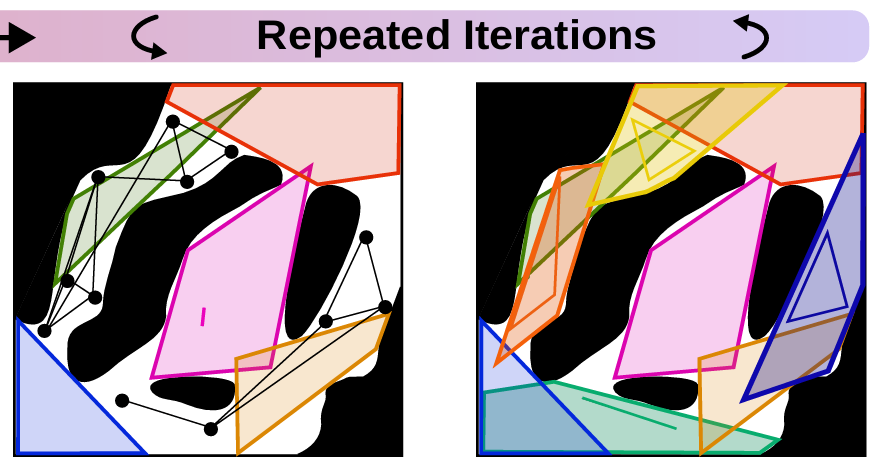
\includegraphics[width=\textwidth]{./imgs/VCC-5.png}

        \column{0.5\textwidth}
        \textbf{Iteration Process:}
        \begin{itemize}
            \item Lấy mẫu mới từ không gian trống còn lại
            \item Lặp lại các bước 1-4 cho vùng chưa phủ
            \item Tiếp tục đến khi đạt độ phủ $\alpha$ đủ
        \end{itemize}

        \vspace{0.5em}
        \textbf{Điều kiện dừng - Quá trình kết thúc khi:}
        \begin{itemize}
            \item Đạt độ phủ mong muốn $\alpha$
            \item Không còn không gian đáng kể để phủ
            \item Số vùng lồi đã đủ cho ứng dụng
        \end{itemize}
    \end{columns}
\end{frame}

\end{document}
